\documentclass[a4paper,12pt]{book}

% Paquetes necesarios
\usepackage[utf8]{inputenc}   % Codificación de caracteres
\usepackage[spanish]{babel}   % Idioma español
\usepackage[T1]{fontenc}      % Codificación de fuentes
\usepackage{amsmath, amssymb} % Símbolos matemáticos
\usepackage{graphicx}         % Inclusión de gráficos
\usepackage{cite}             % Gestión de citas
\usepackage{hyperref}         % Enlaces y referencias
\usepackage{geometry}         % Configuración de márgenes
\usepackage{fancyhdr}         % Encabezados y pies de página
\usepackage{titlesec}         % Formato de títulos
\usepackage{booktabs}         % Tablas profesionales
\usepackage{caption}          % Personalización de leyendas
\usepackage{enumitem}         % Personalización de listas
\usepackage{float}
\usepackage{tcolorbox}
\usepackage[table]{xcolor} % Paquete para colores en tablas
\usepackage{colortbl}       % Complemento para colorear celdas específicas
\usepackage{multirow}       % Combinar celdas en tablas
\usepackage{makecell}       % Combinar celdas en tablas
\usepackage{enumitem}
\usepackage{amsmath}
\usepackage{eurosym}
\usepackage{tikz}
\usepackage{pdfpages}




\newcommand{\cuenta}[1]{
    \ifnum#1=2800 2800. Amortización acumulada de investigación\fi
    \ifnum#1=251 251. Valores representativos de deuda\fi
    \ifnum#1=250 250. Inversiones financieras a l/p en instrumentos de patrimonio\fi
    \ifnum#1=133 133. Ajustes en la valoración en AF a VR[PN]\fi
    \ifnum#1=900 900. Beneficios en AF a VR[PN]\fi
    \ifnum#1=7632 7632. Beneficios en AR a VR [PN] \fi
    \ifnum#1=802 802. Transferencias de Beneficios en AR a VR [PN]\fi
    \ifnum#1=766 766. Beneficios en participaciones y VRD\fi
    \ifnum#1=800 800. Pérdidas en AR a VR[PN]\fi
    \ifnum#1=761 761. Ingresos de valores representativos de deuda\fi
    \ifnum#1=546 546. Intereses a corto plazo de valores representativos de deuda\fi
    \ifnum#1=572 572. Bancos c/c \fi
    \ifnum#1=541 541. Valores representativos de deuda a corto plazo \fi
    \ifnum#1=669 669. Otros gastos financieros\fi
    \ifnum#1=666 666. Pérdidas en participaciones y VRD\fi
    \ifnum#1=540 540. Inversiones financieras c/p en instrumentos de patrimonio\fi
    % \ifnum#1=\fi
    % \ifnum#1=\fi
    % \ifnum#1=\fi
    % \ifnum#1=\fi
    % \ifnum#1=\fi
    % \ifnum#1=\fi
    % \ifnum#1=\fi
    % \ifnum#1=\fi
    % \ifnum#1=\fi
    % \ifnum#1=\fi
}
\renewcommand{\c}[1]{\textit{#1}}
\newcommand{\p}{\text{.}}


% Configuración de márgenes
\geometry{left=3cm, right=3cm, top=2.5cm, bottom=2.5cm}

% Configuración de encabezados y pies de página
% \setlength{\headheight}{14.49998pt}
\pagestyle{fancy}
\fancyhf{}
\fancyhead[L]{Universidad de Granada}
\fancyhead[L]{\nouppercase{\leftmark}}

% \fancyhead[C]{Escuela Técnica Superior de Ingenierías Informática}
%\fancyhead[L]{Universidad de Granada}
\fancyhead[R]{Contabilidad Financiera II}
\fancyfoot[L]{\rule[0pt]{\textwidth}{0.2pt}\\Ismael Sallami Moreno}
\fancyfoot[C]{\rule[0pt]{\textwidth}{0.2pt}\\\thepage}
\fancyfoot[R]{\rule[0pt]{\textwidth}{0.2pt}\\\today}
\renewcommand{\sectionmark}[1]{\markboth{#1}{}} % Configura \leftmark para que solo muestre la sección

% Formato de títulos
\titleformat{\section}{\large\bfseries}{\thesection.}{0.5em}{}
\titleformat{\subsection}{\normalsize\bfseries}{\thesubsection.}{0.5em}{}

% Datos del documento
\title{\textbf{Práctica Contabilidad Financiera II}}
\author{
    Ismael Sallami Moreno \\
    \texttt{ism350zsallami@correo.ugr.es}
}
\date{
    \vspace{1cm}
    \begin{tabular}{rl}
        \textbf{Asignatura:} & Contabilidad Financiera II \\
        \textbf{Tema:} & Práctica \\
        \textbf{Fecha:} & \today
    \end{tabular}
}

\begin{document}

% Portada
\begin{titlepage}
    \begin{center}
        % \vspace*{1cm}
        
        % \Huge
        % \textbf{Práctica Contabilidad Financiera II}
        \Huge \textbf{Práctica Contabilidad Financiera II} 
        % \vspace{0.5cm}
        % \LARGE
        % \textbf{Ismael Sallami Moreno}\\
        % \LARGE
        % \texttt{ism350zsallami@correo.ugr.es}
        % \LARGE
        % \url{https://github.com/Ismael-Sallami}
        
        % \vfill
        
        % \Large
        % \textbf{Universidad de Granada}
        
        \vspace{0.8cm}
        
        \begin{tikzpicture}[remember picture, overlay]
            \node[opacity=0.2] at (current page.center) {
\includegraphics[width=\paperwidth,height=\paperheight]{portada.jpg}};
            \node[align=center] at (current page.center) {
                
                \vspace{0.5cm}
                \LARGE \textbf{Ismael Sallami Moreno} \\
                \LARGE \texttt{ism350zsallami@correo.ugr.es} \\
                \LARGE \url{https://ismael-sallami.github.io/} \\
                \LARGE \url{https://elblogdeismael.github.io/} \\
                \vspace{2cm}
                \Large \textbf{Universidad de Granada} \\
                \vspace{0.8cm}
                % \Large \textbf{2025}
            };
        \end{tikzpicture}
        \vfill
        
        \Large
        \textbf{2025}
        
    \end{center}
\end{titlepage}
\newpage

% Resumen
% \begin{abstract}
% \noindent
% \textbf{Resumen:} Este documento presenta los apuntes y/o resúmenes del tema que se expone que se han realizado a lo largo del curso de la asignatura de Inteligencia Artificial. En este caso, se trata de las prácticas de la asignatura.
% \end{abstract}
% \bigskip


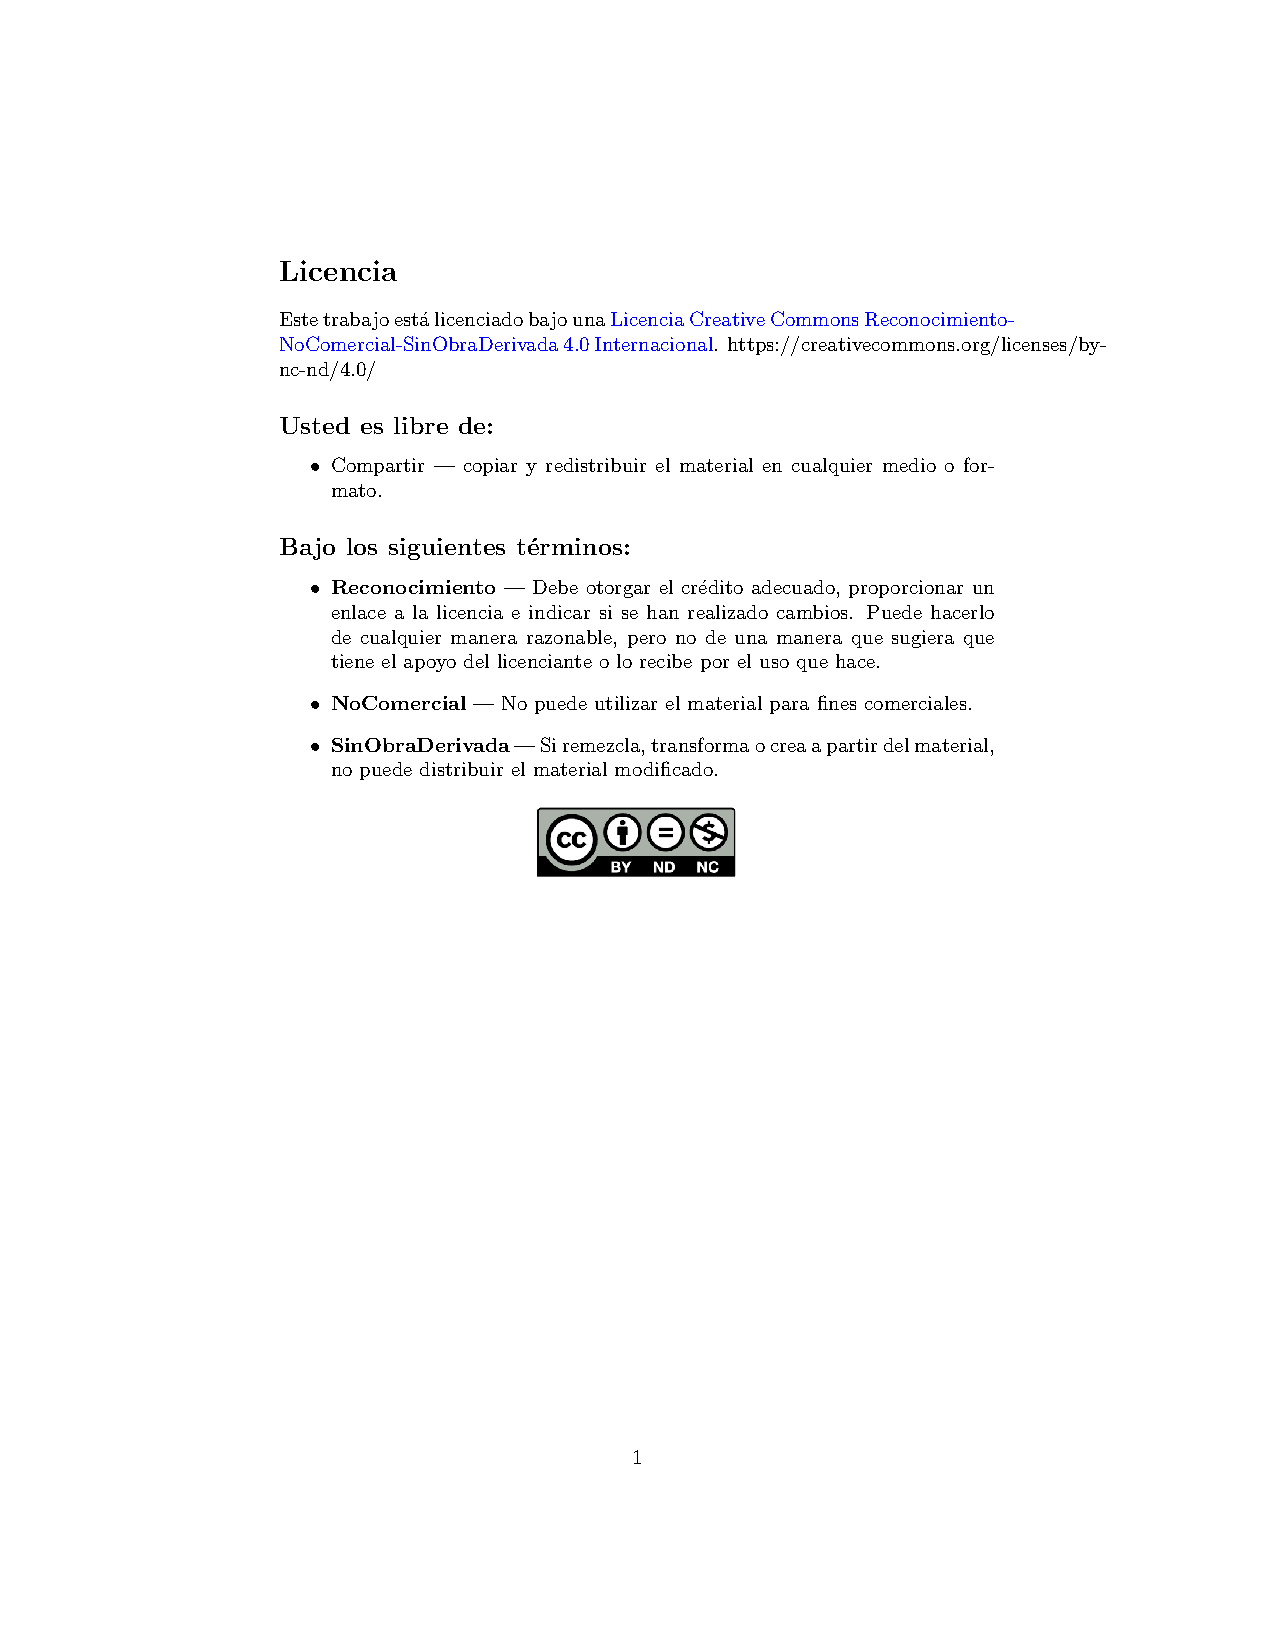
\includepdf[pages=-]{../../../../extraFiles/licencia.pdf}
% Tabla de contenidos
\tableofcontents
\newpage

\chapter{Activos Financieros}

\section{Ejercicios}

\subsection*{Ejercicio 1 }

\begin{enumerate}
    \item En el Boletín de Deuda Pública del día 23 de marzo de 2012, en su sección de operaciones de compraventa simple al contado sobre Deuda del Estado, podemos encontrar la siguiente información:
    
    \begin{table}[h!]
        \centering
        \begin{tabular}{|c|c|c|c|c|}
            \hline
            \textbf{EMISIÓN} & \textbf{Cupón} & \textbf{Amortización} & \textbf{Precio medio ex cupón} & \textbf{TIR} \\
            \hline
            ES00000123B9 O EST & 5.50 & 30.04.21 & 101,105 & 5,34 \\
            \hline
        \end{tabular}
    \end{table}

    \begin{tikzpicture}
        % Línea de tiempo
         \draw[-] (0,0) -- (12,0) node[right] {Tiempo};
    
        % Emisión inicial
        \draw[-{Latex}] (0,0) -- (0,-1) node[below right, yshift=-0.5cm, xshift=-1.5cm, align=center, text width=3cm] {30/04/12\\Emisión\\1000};
    
        % Pagos periódicos
        \draw[-{Latex}] (2,0) -- (2,1) node[above, yshift=0.4cm, align=center, text width=3cm] {30/04/14};
        \draw[-{Latex}] (4,0) -- (4,1) node[above, yshift=0.4cm, align=center, text width=3cm] {30/04/15};
        \draw[-{Latex}] (6,0) -- (6,1) node[above, yshift=0.4cm, align=center, text width=3cm] {...};
        \draw[-{Latex}] (12,0) -- (12,1) node[above, yshift=0.4cm, align=center, text width=3cm] {30/04/21\\};
    
        % % Emisión final
        % \draw[-{Latex}] (11.8,0) -- (11.8,-1) node[below right, yshift=-0.5cm, xshift=-1.5cm, align=center, text width=3cm] {30/04/21\\};
    
    
    
        % Conversión
        % \draw[-{Latex},red] (3,0) -- (3,-1) node[below left, yshift=-0.8cm, xshift=-0.3cm, align=center, text width=3cm] {31/3/06\\Conversión};
    
        % % Venta
        % \draw[-{Latex},blue] (3.5,0) -- (3.5,1) node[above, yshift=0.8cm, align=center, text width=3cm] {30/4/06\\Venta};
    
        % % Amortización final
        % \draw[-{Latex}] (10,0) -- (10,-1) node[below right, yshift=-0.8cm, xshift=0.3cm, align=center, text width=3cm] {31/12/09\\Amortización\\1020};
    
    \end{tikzpicture}
    
    \begin{enumerate}
        \item[a)] Si se supone que se ha comprado esta obligación por el precio medio, ¿Cuánto se ha pagado por ella? \textbf{Sol: 1.060,34€}
        
        \begin{itemize}
            \item Del 30/04/11 al 23/03/12 hay 328 días.
            \item Del 23/03/12 al 30/04/12 hay 38 días.
            \item El total es de 366 días.
        \end{itemize}

        \begin{equation*}
            P_{\text{total}} = 101,105 \times 1000 + \frac{55}{366} \times 328 = 1.060,34
        \end{equation*}
        \item[b)] Plantea la ecuación que verifica la TIR con la que se está contratando esta obligación y calcula su valor. \textbf{Sol: 5,34\%}
        \begin{equation*}
            1060,34 = \left[55 \times a_{10,TIR}+\frac{1000}{(1+TIR)^{10}}\right]\times(1+TIR)^{\frac{328}{366}}
        \end{equation*}
    \end{enumerate}
\end{enumerate}

\textit{Debemos de hacer ciertas suposiciones como es el caso de que al amortizarse en 30.04.21, y estamos a 23.03.12, el comienzo de la vida de la obligación es el 30.04.12.}
\\\\

% \begin{tikzpicture}
%     % Línea de tiempo
%      \draw[-] (0,0) -- (12,0) node[right] {Tiempo};

%     % Emisión inicial
%     \draw[-{Latex}] (0,0) -- (0,-1) node[below right, yshift=-0.5cm, xshift=-1.5cm, align=center, text width=3cm] {30/04/12\\Emisión\\1000};

%     % Pagos periódicos
%     \draw[-{Latex}] (2,0) -- (2,1) node[above, yshift=0.4cm, align=center, text width=3cm] {30/04/14};
%     \draw[-{Latex}] (4,0) -- (4,1) node[above, yshift=0.4cm, align=center, text width=3cm] {30/04/15};
%     \draw[-{Latex}] (6,0) -- (6,1) node[above, yshift=0.4cm, align=center, text width=3cm] {...};
%     \draw[-{Latex}] (12,0) -- (12,1) node[above, yshift=0.4cm, align=center, text width=3cm] {30/04/21\\};

%     % % Emisión final
%     % \draw[-{Latex}] (11.8,0) -- (11.8,-1) node[below right, yshift=-0.5cm, xshift=-1.5cm, align=center, text width=3cm] {30/04/21\\};



%     % Conversión
%     % \draw[-{Latex},red] (3,0) -- (3,-1) node[below left, yshift=-0.8cm, xshift=-0.3cm, align=center, text width=3cm] {31/3/06\\Conversión};

%     % % Venta
%     % \draw[-{Latex},blue] (3.5,0) -- (3.5,1) node[above, yshift=0.8cm, align=center, text width=3cm] {30/4/06\\Venta};

%     % % Amortización final
%     % \draw[-{Latex}] (10,0) -- (10,-1) node[below right, yshift=-0.8cm, xshift=0.3cm, align=center, text width=3cm] {31/12/09\\Amortización\\1020};

% \end{tikzpicture}

% \begin{itemize}
%     \item Del 30/04/11 al 23/03/12 hay 328 días.
%     \item Del 23/03/12 al 30/04/12 hay 38 días.
%     \item El total es de 366 días.
% \end{itemize}
% Así que calculando el precio total con la fórmula del precio excupón tenemos que:
% \begin{itemize}
%     \item [a)] \begin{equation*}
%         P_{\text{total}} = 101,105 \times 1000 + \frac{55}{366} \times 328 = 1.060,34
%     \end{equation*}


%     \item [b)] \begin{equation*}
%         1060,34 = \left[55 \times a_{10,TIR}+\frac{1000}{(1+TIR)^{10}}\right]\times(1+TIR)^{\frac{328}{366}}
%     \end{equation*}
% \end{itemize}


\subsection*{Ejercicio 2}

\begin{enumerate}
    \item La sociedad ILIGRASA emitió, el 1 de enero de 2011, obligaciones con:
    \begin{itemize}
        \item Valor nominal de 3.000€.
        \item Cupón al 5\% nominal anual pagadero por semestres (30 de junio y 31 de diciembre de cada año).
        \item Vencimiento a 10 años.
    \end{itemize}
    Los títulos se emitieron a la par sin gastos para el suscriptor. Hoy, 21 de junio de 2013, estos títulos cotizan en el mercado secundario al 108\% excupón.

    \begin{enumerate}
        \item[a)] Plantea la ecuación que verifica la rentabilidad que el mercado exige hoy a estos títulos y calcula su valor. \textbf{Sol: 3,7997\%.}
        Como primer paso debemos de calcular el $C_s$, el cual nos queda $C_s = \frac{5\%}{2} \times 3000 = 75$\footnote{Se divide entre 2 porque el pago es semestral y me dan el tipo de interés anual.}. 

        A continuación, caculamos el precio total, el cual nos queda:
        \begin{equation*}
            {P_T}_{\textit{21.06.13}} = 108\% \times 3000 + \frac{75}{181} \times 172 = 3311,27
        \end{equation*}

        Por lo que teniendo en cuenta que los días que han pasado desde el último pago son 172, podemos plantear la ecuación de la rentabilidad que el mercado exige hoy a estos títulos:

        \begin{equation*}
            3311,27 = \left[75 + a_{16,TIR_semestral} + \frac{3000}{(1+TIR)^{16}}\right] \times (1+TIR)^{\frac{172}{181}}
        \end{equation*}
        \item[b)] Si un inversor compró 15 títulos en la emisión y los vende hoy a través de un intermediario, cobrándole éste una comisión del 0,3\% sobre el valor efectivo de la venta, ¿qué rentabilidad efectiva ha obtenido con ellos? \textbf{Sol: 8,0361\%.}\\\\
        Se emitió a la par, por lo que es igual a el VN.
        El precio de venta es $ P_{venta} = 3311,27 -0,3 \times 3311,27 = 3301,34$

        La rentabilidad efectiva es:
        \begin{equation*}
            3000 = 75 \times a_{4,TIR} + \frac{3301,34}{1+TIR}^{\alpha}
        \end{equation*}

        Donde $\alpha$ es:
        \begin{align*}
            \alpha = \frac{4s+1ts = 172\text{días}+4s}{181}
        \end{align*}
        Donde denotamos s como semestre y ts como un trozo del simestre.
    \end{enumerate}
\end{enumerate}


\subsection*{Ejercicio 3}

El 1 de enero de 2011, cierta sociedad realizó una emisión de obligaciones con valor nominal unitario de 6.000€, cupón trimestral al 6\% nominal y vencimiento a 10 años. La emisión se realizó a la par e incluía una cláusula de rescate anticipado con un precio de rescate igual al 110\% del valor nominal de la obligación más el cupón corrido correspondiente. Hoy, 16 de abril de 2013, la rentabilidad que exige el mercado para estas obligaciones es del 4\% nominal.

Podemos representar la casuísitca de la siguiente manera:

\begin{tikzpicture}
    % Línea de tiempo
    \draw[-] (0,0) -- (12,0) node[right] {Tiempo};

    % Fechas
    \draw[-{Latex}] (0,0) -- (0,-1) node[below, yshift=-0.5cm, align=center, text width=3cm] {01/01/11\\Emisión};
    \draw[-{Latex}] (1,0) -- (1,-1) node[below, yshift=0cm, align=center, text width=3cm] {/12};
    \draw[-{Latex}] (2,0) -- (2,-1) node[below, yshift=0cm, align=center, text width=3cm] {/13};
    \draw[-{Latex}] (4,0) -- (4,-1) node[below, yshift=-0.5cm, align=center, text width=3cm] {1/04/13};
    \draw[-{Latex}] (6,0) -- (6,-1) node[below, yshift=-0.5cm, align=center, text width=3cm] {\textcolor{red}{16/04/13}};
    \draw[-{Latex}] (9.3,0) -- (9.3,-1) node[below, yshift=-0.5cm, align=center, text width=3cm] {/14};
    \draw[-{Latex}] (10,0) -- (10,-1) node[below, yshift=-0.5cm, align=center, text width=3cm] {...};
    \draw[-{Latex}] (8,0) -- (8,-1) node[below, yshift=-0.5cm, align=center, text width=3cm] {21/06/13};
    \draw[-{Latex}] (12,0) -- (12,-1) node[below, yshift=-0.5cm, align=center, text width=3cm] {30/04/21\\Vencimiento};
\end{tikzpicture}



\begin{enumerate}
    \item[a)] Calcula el precio de cotización de estas obligaciones hoy.
    
    \begin{align*}
        P_T = P_{\text{excupón}} + CC 
    \end{align*}

    \begin{center}
        \begin{tikzpicture}
            % Línea de tiempo
            \draw[-] (0,0) -- (12,0) node[right] {Tiempo};
    
            % Fechas
            \draw[-{Latex}] (0,0) -- (0,-1) node[below, yshift=-0.5cm, align=center, text width=3cm] {01/04/13};
            \draw[-{Latex}] (6,0) -- (6,-1) node[below, yshift=-0.5cm, align=center, text width=3cm] {16/04/13};
            \draw[-{Latex}] (12,0) -- (12,-1) node[below, yshift=-0.5cm, align=center, text width=3cm] {01/07/13};
    
            % Línea de días
            \draw[|-|] (0,-2.7) -- (6,-2.7) node[midway, below] {15 días};
            \draw[|-|] (0,-4) -- (12,-4) node[midway, below] {91 días};
        \end{tikzpicture}
    \end{center}

    \begin{align*}
        \text{Cupón} = \frac{6\%}{4} \times 6000 = 90 \\
        \text{CC}_{16/04/13} = \frac{90}{91} \times 15 = 14,84 \\
        n = 10 \times 4 - 9 (\text{ ya han pasado })= 31 \text{ trimestres } \\
        P_T = \left[63,3 \times a_{31,0'01} + \frac{6000}{1,01^{31}}\right] \times 1,01^{16/91} = 6807,42\\
        P_{\text{cotización = excupón}} = P_T - CC = 6807,42 - 14,84 = 6792,58
    \end{align*}

    Para saber la cotización $\rightarrow \frac{6792,58}{6000} \times 100 = 113,21\%$



    \item[b)] ¿Es conveniente para la sociedad emisora rescatar las obligaciones hoy? Razona la respuesta.

    Sí ya que cotiza a 6792,58 y si lo rescato es: $110\% \times 6000 + CC = 6600 + 14,84 = 6614,84$.

    Como 6614,84 < 6807,42, es conveniente rescatarlas ya que puedo comprar más barato de lo que cotiza en el mercado.


    \item[c)] ¿Qué rentabilidad efectiva obtendría un inversor que compró 10 obligaciones en la emisión si se las rescataran hoy?
    
    \begin{equation*}
        6000 = 90 \times a_{9,TIR} + \frac{6614,84}{1+TIR}^{9+15/91}
    \end{equation*}

    \begin{equation*}
        (1 + TIR_t)^4 = 1 + TIR_{\text{anual}} \Rightarrow TIR_a = 10,322\%
    \end{equation*}

\end{enumerate}

\subsection*{Ejercicio 4}

Un inversor compra 750 obligaciones convertibles de una sociedad, de nominal 10.000 u.m. y cupón al 12 \% nominal pagadero por semestres en las fechas de 31 de mayo y 30 de noviembre. La compra se efectúa el 30 de junio al precio del 95 \% más cupón corrido. El 30 de julio se convierten las obligaciones en acciones. Las obligaciones se valoran al nominal más el cupón corrido correspondiente. Las acciones, de valor nominal 10 u.m., se cotizan minorando el precio medio en Bolsa del trimestre anterior, 1.500 u.m. (30 \%), en un 15 \%. En la conversión se redondea por exceso el número de acciones, si fuese necesario, aportando el obligacionista la diferencia correspondiente en metálico. Las acciones se admiten a cotización el 1 octubre y se venden el 30 del mismo mes al 320 \%. SE PIDE:
% \begin{enumerate}
%     \item[a)] Importe desembolsado en la compra de los títulos el 30 de junio.
%     \item[b)] Número de acciones obtenidas en la conversión de las obligaciones el 30 de julio.
%     \item[c)] Rentabilidad obtenida en base anual con la venta de las acciones el 30 de octubre.
% \end{enumerate}

% \begin{enumerate}
%     \item[a)] \textbf{Importe desembolsado en la compra de los títulos el 30 de junio.}
    
%     \begin{align*}
%         VN &= 10.000 \\
%         \text{Obligaciones} &= 750 \\
%         C_s &= \frac{12 \%}{2} \times 10.000 = 600 \\
%         \text{Precio de compra} &= 95\% \times 10.000 + 600 = 9.500 + 600 = 10.100 \\
%         \text{Total desembolsado} &= 10.100 \times 750 = 7.198.770
%     \end{align*}
    
%     \item[b)] \textbf{Número de acciones obtenidas en la conversión de las obligaciones el 30 de julio.}
    
%     \begin{align*}
%         B &= 10.000 + \frac{}{} = 10.600 \\
%         A &= 1500 - 15\% \times 1500 = 1275 \\
%         \text{Tasa de conversión} &= \frac{B}{A} = \frac{10.600}{1275} \approx 8,31 \text{ acciones/obligación} \\
%         \text{Total acciones} &= 8 \times 750 = 6.000 \text{ acciones}
%     \end{align*}
    
%     \item[c)] \textbf{Rentabilidad obtenida en base anual con la venta de las acciones el 30 de octubre.}
    
%     \begin{align*}
%         \text{Precio de venta} &= 320\% \times 500 = 1.600 \\
%         \text{Total obtenido} &= 6.000 \times 1.600 = 9.600.000 \\
%         i &= \frac{9.600.000}{7.198.770} - 1 \\
%         &= \left(1 + i \times \frac{120}{360}\right) \\
%         i &= 100 \% \\ 
%         7\p198\p770 = \frac{9\p600\p000}{\left(1 + i \times \frac{120}{360}\right)} \\
%     \end{align*}
    
% \end{enumerate}

\begin{enumerate}
    \item[a)] Importe desembolsado en la compra de los títulos el 30 de junio.
    
    \begin{align*}
        C_s = 6\% \times 10\p000 = 600 \\
        P_T = P_{\text{excupón}} + CC = \\
        = 6\p000 \times 95\% + \frac{600}{183} \times 30 = 9598,36 \\
        \text{Total desembolsado} = 9598,36 \times 750 = 7\p198\p770
    \end{align*}

    \item[b)] Número de acciones obtenidas en la conversión de las obligaciones el 30 de julio.
    
    \begin{align*}
        \text{Tasa de conversión} = \frac{B}{A} \\
        B = 10\p000 + \frac{600}{183} \times 60 = 10\p196,72 \\
        A = 1500 - 15\% \times 1500 = 1275 \\
        \text{Tasa de conversión} = \frac{10\p196,72}{1275} \approx 7,9974 \rightarrow \\ \rightarrow 8 \text{ acciones/obligación} \times 750 \text{ obligaciones}= 5998, 0706 \text{ acciones}
\end{align*}

    \item[c)] Rentabilidad obtenida en base anual con la venta de las acciones el 30 de octubre.
    
    \begin{itemize}
        \item Cada acción se vende a 320\% $\rightarrow 320\% \times 500 \text{ €/acción } = 1600 \text{ €/acción}$
    \end{itemize}

    \begin{align*}
        7\p198\p770 = \frac{9\p600\p000}{(1 + i \times \frac{120}{360}) \rightarrow i = 100\%}
    \end{align*}

    \textit{Se usa 120 en vez de 118 para coger los 4 meses completos, es decir,para conseguir calculos más exactos.}

\end{enumerate}


\subsection*{Ejercicio 5}

El 27 de marzo de 2016 una empresa realizó una emisión de obligaciones convertibles a 3 años, de valor nominal 1.000 euros, emisión a la par y cupón anual del 5 \%. En el folleto de emisión se establece que estos títulos pueden ser convertidos voluntariamente (por parte de los inversores) en acciones de la compañía emisora el 27 de marzo de 2017, siendo el valor de la obligación a efectos de conversión el nominal y la tasa de conversión de las obligaciones (esto es, el número de acciones que corresponda a cada obligación) de 200. Además, las obligaciones incluyen una cláusula de rescate anticipado a favor del emisor al 110 \%. Un mes antes de la fecha de conversión, la empresa emisora anunció que ejercería su cláusula de rescate anticipado el 27/03/2017 si los obligacionistas no optan por la conversión. SE PIDE:
\begin{enumerate}
    \item[a)] Suponga que hoy, día 27 de marzo de 2017, las acciones de la empresa cotizan a 6€/acción. Indique si interesa o no a los obligacionistas acudir a la primera conversión, especificando el precio de las acciones para la conversión y el valor de la conversión. Comente los resultados obtenidos.
    
    \begin{align*}
        \text{Precio por acción }  =\frac{1000}{200} = 5 \\
        \text{Valor de la conversión } = 200 \times 6 = 1200
    \end{align*}

    Vemos que si interesa, ya que el valor de la acción hoy es de 6€ y el valor de la conversión es de 1200€, por lo que se obtiene un beneficio de 200€.

    \item[b)] Teniendo en cuenta el escenario planteado en el apartado a) suponga que el inversor A adquirió las obligaciones en la emisión, las convirtió en acciones el 27 de marzo de 2017 y decide venderlas el 27 de mayo de 2017 cuando cotizan a 5,25 €/acción. Plantee la ecuación para calcular la rentabilidad efectiva de este inversor.
    
    \begin{tikzpicture}
        % Línea de tiempo
        \draw[-] (0,0) -- (10,0) node[right] {Tiempo};

        % Fechas
        \draw[-{Latex}] (0,0) -- (0,-1) node[below, yshift=-0.5cm, align=center, text width=3cm] {27/03/17};
        \draw[-{Latex}] (10,0) -- (10,-1) node[below, yshift=-0.5cm, align=center, text width=3cm] {25/05/17\\Cotizan a 5,25};

        % Línea de días
        \draw[|-|] (0,-3) -- (10,-3) node[midway, below] {4 + 27 + 30 = 61 días};
    \end{tikzpicture}
    
    Si las vendemos las acciones aquí obtenemos $200 \times 5,25 = 1050$.


    La ecuación de la rentabilidad nos queda:
    \begin{equation*}
        1050 = \frac{50}{1+R} + \frac{50}{(1+R)^{61/365}}
    \end{equation*}


    \item[c)] Suponga ahora que hoy, día 27 de marzo de 2017, las acciones de la empresa cotizan a 4€/acción y que la rentabilidad que exige el mercado para las obligaciones de la empresa es del 3 \%. Indique si los obligacionistas estarían interesados en acudir a la conversión y si a la empresa emisora le favorece realizar el rescate anticipado. Razone sus respuestas.
    
    No, debido a que 4€/acción < 5€/acción, siendo el valor de la conversión $4\times200 = 800$.

    \begin{align*}
        P_{t\text{ (27/03/17)}} = 50 \times a_{2,3\%} + \frac{1000}{(1+0,03)^2} = 1328,27 \\
        \rightarrow \text{siendo }a_{2,3\%} = \frac{1-(1+i)^{-n}}{i} = 1,913
    \end{align*}

    El rescate anticipado nos queda: 
    \begin{align*}
        1000 \times 1,1 = 1100
    \end{align*}

    Podemos concluir recalcar que no interesa a los obligacionistas acudir a la conversión.


    \item[d)] Teniendo en cuenta el escenario planteado en el apartado c) suponga que el inversor B adquirió las obligaciones 10 días después de la emisión cuando cotizaban al 100,25 \% y se las rescatan el 27 de marzo de 2017. Calcule la rentabilidad efectiva de este inversor.
    
    \begin{align*}
        P_{t\text{ excupón en t = 6/4/16}} = P_{\text{cotización}} \text{ ... } = 1000 \times 1,0025 = 1002,5 \\
        P_{t\text{ (27/03/17) + 10 días}} = 1002,5 + \frac{50}{365} \times 10 = 1003,869 \\
        1003,869 = \frac{1100 + 50}{(1+R)^{\frac{355}{365}}} \rightarrow \\
        \rightarrow R = \left[\frac{1150}{1003,869}\right]^{365/355} - 1 = 14,99 \approx 15\%
    \end{align*}

\end{enumerate}

\subsection*{Ejercicio 6}

Un inversor adquiere el 11 de abril de 2012 un bono del Estado a 3 años, tipo cupón del 4,4\% anual, vencimiento 31/01/2015. El precio ex-cupón fue del 103,992\% y la TIR del 2,89\%.

\begin{enumerate}[label=\textbf{\alph*)}]
    \item Determine el precio pagado por la obligación.
    
    \begin{align*}
        C_a = 4,4\% \times 1000 = 44 \\
        P_t = P_{\text{excupón}} + CC \\
        P_{\text{excupón}} = 103,992\% \times 1000 = 1039,92 \\
        \text{Los días que pasan son } 70 = 31 + 28 + 31 \\
        CC = \frac{44}{365} \times 70 = 8,44
    \end{align*}

    Nos queda:
    \begin{align*}
        \Rightarrow P_t = 1039,92 + 8,44 = 1048,36
    \end{align*}

    \item Plantee la ecuación que verifica la TIR con la que se está comprando este bono.
    
    \begin{align*}
        1048,36 = \left[44 \times a_{3, TIR} + \frac{1000}{(1+TIR)^3}\right] \times (1+TIR)^{\frac{70}{365}}
    \end{align*}

    \item Calcule la duración del bono en el momento de la emisión (31/01/2012), suponiendo que la TIR a esa fecha coincide con el cupón pagado por el bono.
    \item En esa misma fecha de emisión, si los tipos de interés bajasen 75 puntos básicos, aproxime a través de la duración modificada cuál sería el nuevo precio del bono.
\end{enumerate}



\subsection*{Ejercicio 7 }

El Tesoro Público recibió las siguientes peticiones competitivas en una subasta de obligaciones del Estado a 10 años, además de 100 millones correspondientes a peticiones no competitivas.

\begin{table}[H]
\centering
\begin{tabular}{|c|c|}
\hline
Nominal (millones €) & Precio solicitado \\ \hline
100                  & 113,975           \\ \hline
200                  & 112,885           \\ \hline
250                  & 111,275           \\ \hline
450                  & 110,000           \\ \hline
400                  & 109,375           \\ \hline
\end{tabular}
\caption{Peticiones competitivas recibidas}
\end{table}

Estas obligaciones, que pagarán un cupón anual del 5,5\%, se emitieron el 30/03/2010 y se amortizarán el 30/03/2020.

\begin{enumerate}[label=\textbf{\alph*)}]
    \item Resuelve la subasta sabiendo que el Tesoro adjudicó un total de 800 millones.\\
    Solución: Precio medio 111,848; Precio marginal 110.

    Sabemos que el total adjudicado es de 800 millones, por lo que podemos plantear la siguiente ecuación:
    \begin{align*}
        \text{Total adjudicado} = 800 M \\
        - PNC = 100 M \\
        = 700 M \\
    \end{align*}

    \begin{table}[h]
        \centering
        \begin{tabular}{p{2cm}p{2cm}p{2cm}p{2cm}}
            \toprule
            \textbf{Precio} & \textbf{Volumen Adjudicado} & \textbf{Volumen Adjudicado Acumulado} & \textbf{Precio Adjudicado}  \\
            \midrule
            113,975&100&100&\\
            112,885&200&300&\\
            111,275&250&550&\\
            110,000&450&700 (sobra)&\\
            \bottomrule
        \end{tabular}
        \caption{Subasta}
        \label{tab:subastaej7}
    \end{table}
    En la tabla \ref{tab:subastaej7} cortamos en 110,000 porque es el precio que nos sobra para llegar a los 800 millones, lo demás ya no entra en la subasta.

    \begin{align*}
        \text{Precio medio} = \\ = \frac{100 \times 113,975 + 200 \times 112,885 + 250 \times 111,275 + 450 \times 110,000}{800} = 111,848
    \end{align*}

    \begin{align*}
        \text{Precio marginal} = 110
    \end{align*}

    El precio marginal es el precio que se ha adjudicado a los 450 millones restantes, es decir, en este caso corresponde al precio de ``corte'' de la subasta.

    \item Plantea la ecuación que verifica el tipo de interés marginal resultante de la subasta.\\
    Solución: 4,2516\%.

    \begin{equation*}
        1100 = 55 \times a_{10,TIR_{marginal}} + \frac{1000}{(1+TIR_{marginal})^{10}}
    \end{equation*}

    En base a la ecuación anterior, cabe destacar que la TIR es menor porque el valor actual es menor que el valor final (1100>1000), por ende, la TIR < 5,5\%.



    \item Si un inversor participó en la subasta solicitando obligaciones a 112,885 y decide venderlas hoy, 09/04/2013, cuando cotizan al 101,245\%, plantea la ecuación que verifica la rentabilidad efectiva obtenida con ellas sabiendo que el intermediario le cobra una comisión en la operación de venta del 0,3\% sobre el nominal.\\
    Solución: 1,7529\%.

    El precio del excupón es 101,245\%, adjudicándose al 111,848\%.
    El cupón es de 55 = $5,5\% \times 1000$.
    La comisión es de 3\%.
    \\\\\\\\
    \begin{tikzpicture}
        % Línea de tiempo
        \draw[-] (0,0) -- (12,0) node[right] {Tiempo};

        % Emisión inicial
        \draw[-{Latex}] (0,0) -- (0,-1) node[below right, yshift=-0.5cm, xshift=-1.5cm, align=center, text width=3cm] {30/03/10\\Emisión\\1000};

        % Pagos de cupones
        \draw[-{Latex}] (2,0) -- (2,1) node[above, yshift=0.4cm, align=center, text width=3cm] {30/03/11\\Cupón\\55};
        \draw[-{Latex}] (4,0) -- (4,1) node[above, yshift=0.4cm, align=center, text width=3cm] {30/03/12\\Cupón\\55};
        \draw[-{Latex}] (6,0) -- (6,1) node[above, yshift=0.4cm, align=center, text width=3cm] {30/03/13\\Cupón\\55};
        \draw[-{Latex}] (8,0) -- (8,1) node[above, yshift=0.4cm, align=center, text width=3cm] {30/03/14\\Cupón\\55};
        \draw[-{Latex}] (10,0) -- (10,1) node[above, yshift=0.4cm, align=center, text width=3cm] {09/04/13\\Precio Venta};
        % \draw[-{Latex}] (10,0) -- (10,1) node[above, yshift=0.4cm, align=center, text width=3cm] {30/03/15\\Cupón\\55};
        % \draw[-{Latex}] (12,0) -- (12,1) node[above, yshift=0.4cm, align=center, text width=3cm] {30/03/20\\Amortización\\1000};

    \end{tikzpicture}

    \begin{align*}
        \text{Precio de Venta} = 1012,45 + \frac{55}{365} \times 10 = 1013,96 \\
        \text{Precio de Venta}_{\text{Neto}} = 1013,96 - 3 = 1010,96
    \end{align*}

    Sabemos que paga por el 1118,48, ya que coincide con la fecha, sino \textit{deberíamos de añadir el cupón corrido}.

    \begin{equation*}
        1118,48 = 55 \times a_{3,TIR} + \frac{1010,96}{(1+TIR)^{3}}
    \end{equation*}

    \item Plantea la ecuación que verifica la rentabilidad que exige el mercado hoy a estas obligaciones.\\
    Solución: 5,2772\%.

    Siendo hoy el 09/04/2013, nos queda:

    \begin{equation*}
        1013,96 = \left(55 \times a_{7,TIR}+\frac{1000}{(1+TIR)^7}\right) \times (1+TIR)^{7+\left[10/365\right]}
    \end{equation*}

\end{enumerate}

\subsection*{Ejercicio 8}

En la última subasta de Letras del Tesoro a 6 meses (182 días), el Banco de España recibió peticiones no competitivas por valor nominal de 423 millones de euros, y las peticiones competitivas que se indican en el cuadro siguiente:

\begin{table}[h]
    \centering
    \renewcommand{\arraystretch}{1.2}
    \begin{tabular}{|p{2cm}|p{1cm}|p{1cm}|p{1cm}|p{1cm}|p{1cm}|p{1cm}|p{1cm}|p{1cm}|p{1cm}|}
        \hline
        \textbf{Volumen (millones €)} & 27 & 175 & 216 & 110 & 70 & 20 & 821 & 1929 & 600 \\
        \hline
        \textbf{Precio (\%)} & 99,335 & 99,135 & 99,118 & 99,112 & 99,102 & 99,1 & 99,03 & 98,725 & 98,615 \\
        \hline
    \end{tabular}
    \caption{Relación entre volumen y precio}
    \label{tab:volumen_precio}
\end{table}


Ante estas peticiones, decidió adjudicar un volumen total de 1.021 millones. Y sabemos que cierta entidad financiera acudió a esta subasta, solicitando nominal por valor de 5 millones de euros al precio del 99,135\%.

Se pide:

\begin{enumerate}[label=\textbf{\alph*)}]
    \item Calcula el tipo de interés marginal de la subasta. \textbf{Sol: 1,793\%}
    
    

    

    \item ¿Qué precio pagó la entidad financiera por las letras conseguidas en la subasta? \textbf{Sol: 99,130}
    \item Si, 20 días después de comprarlas, la entidad vende las letras en el mercado secundario al interés del 1,5\%, ¿qué rentabilidad efectiva consiguió con estas letras, suponiendo base 360 días? \textbf{Sol: 3,689\%}
\end{enumerate}

\subsection*{Ejercicio 9}

Cierta empresa decide financiarse a corto plazo, 20 días, mediante una operación simultánea sobre pagarés de empresa a un año (360 días) que tiene en su cartera. Estos pagarés, de nominal 6.000€ y que vencen dentro de 245 días, se compraron en la emisión al 96,975\%. La operación simultánea consiste en vender hoy pagarés al 97,125\% y comprarlos dentro de 20 días al 97,425\%.

\begin{enumerate}[label=\textbf{\alph*)}]
    \item Si las letras del tesoro a un año que se emitían en la misma fecha ofrecían un 1,5\% de rentabilidad, ¿con qué prima de riesgo se emitieron estos pagarés?
    
    Sabiendo que la tasa libre de riesgo es del 1,5\% y que se compraron en la emisión al 96,975 \%, podemos plantear la siguiente ecuación:

    % \begin{align*}
    %     VN = 6\p000 \\
    %     i = 1,5\% = rf = \text{tasa libre de riesgo}\\
    %     \text{riesgo pagarés} = rf + \text{Prima de riesgo} \\ 
    %     96,975 = \frac{1000}{1 + i_{\text{pagarés}}} \\
    % \end{align*}

    \begin{equation*}
        96,975 = \frac{100}{1 + i_{\text{pagarés}}} \Rightarrow i_{\text{pagarés}} = 3,12\%
    \end{equation*}

    \[\text{Prima de riesgo} = 3,12\% - 1,5\% = 1,62\%\]


    \item ¿Sobre cuántos pagarés se deberá realizar la operación simultánea si la empresa necesita financiación por valor de 60.000€?
    
    \begin{align*}
        \text{Fuente}_{\text{Hoy}} = 60\p000 \times 97,125\% = 5\p827,5 \\
        \text{Necesitamos } \rightarrow \frac{60\p000}{5827,5} = 10,29 \text{ pagarés} \rightarrow 11 \text{ pagarés}
    \end{align*}

    \item ¿Qué rentabilidad exige el mercado en las operaciones de venta y de compra de la operación simultánea?
    
    \begin{align*}
        5\p825,5 = \frac{6\p000}{1+i\times\times\frac{245}{360}} \Rightarrow i = 4,3495\% \text{(Venta)}\\
    \end{align*}

    \begin{align*}
        \text{Fuente}_{\text{Dentro de 20 días}} = 60\p000 \times 97,425\% = 5\p845,5 \\
        5\p845,5 = \frac{6000}{1+i\times \frac{225}{360}} \Rightarrow i = 4,2289\% \text{(Compra)}
    \end{align*}

    \item ¿Cuál ha sido el coste efectivo de la financiación (Base/365)?
    
    \begin{equation*}
        5827,5 = \frac{5845,6}{(1+TIR)^{\frac{20}{365}}} \Rightarrow TIR = 5,79\%
    \end{equation*}

\end{enumerate}


\subsection*{Ejercicio 10}
En el cuadro adjunto se presentan algunos de los datos correspondientes a la última subasta de letras del tesoro a doce meses:
   
    
    \begin{table}[h!]
        \centering
        \begin{tabular}{|c|c|}
            \hline
            \textbf{LETRAS A 12 MESES (364 días)} & \textbf{} \\
            \hline
            Fecha de liquidación & 20-abr-12 \\
            \hline
            Fecha de vencimiento & 19-abr-13 \\
            \hline
            Precio mínimo aceptado & 97,307 \\
            \hline
            Precio medio & 97,417 \\
            \hline
        \end{tabular}
    \end{table}

    \begin{enumerate}
        \item[a)] Si usted realizó una petición no competitiva para adquirir una letra, indique el precio que pagó por la misma así como el tipo de interés correspondiente (utilice capitalización simple, base 360 y 364 días hasta el vencimiento).
        
        \item[b)] El día 20 de abril de 2012 el precio a plazo de 180 días de las letras es de 98,50\%, y la tasa libre de riesgo es del 2,5\% anual. Explique cómo se podría obtener beneficio sin asumir ningún riesgo aprovechando la oportunidad de arbitraje que se presenta entre el mercado de contado y el mercado a plazo. Cuantifique esa ganancia. Vendiendo al contado y comprando a plazo, 1,35€.
    \end{enumerate}

    \subsection*{Ejercicio 11}

    Los datos de la subasta de Letras del Tesoro a 18 meses celebrada el 15 de enero de 2013 fueron los siguientes:

    \begin{table}[h!]
        \centering
        \begin{tabular}{|c|c|}
            \hline
            \textbf{LETRAS A 18 MESES} & \textbf{ } \\
            \hline
            Fecha de liquidación & 18-ene-13 \\
            \hline
            Fecha de vencimiento & 20-jun-2014 \\
            \hline
            Nominal solicitado & 6.791,24 \\
            \hline
            Nominal adjudicado & 2.509,03 \\
            \hline
            Precio mínimo aceptado & 97,480 \\
            \hline
            Precio medio & 97,622 \\
            \hline
        \end{tabular}
    \end{table}

    \begin{enumerate}
        \item[a)] Determine los tipos de interés marginal y medio de la subasta. \textbf{Sol: medio: 1,687\% marginal: 1,7896\%}
        \item[b)] Si un inversor solicitó letras por valor nominal de 10.000 euros a un precio del 97,5\%, indique a qué precio le fueron adjudicadas las letras, el importe pagado por las mismas y su rentabilidad si las mantiene hasta el vencimiento. \textbf{Sol: 97,5\%, 9.750€, 1,80\%}
        \item[c)] Si el inversor anterior vende las letras transcurridos 200 días, cuando el tipo de interés de mercado es del 2\%, indique la rentabilidad de su inversión. \textbf{Sol: 1,435\%}
        \item[d)] El día 18 de enero de 2013 el precio a plazo de estas letras, fecha de liquidación 60 días después, es del 98,30\%. Si el tipo de interés libre de riesgo anual es del 1,4\%, indique si el inversor del apartado b) puede realizar alguna operación de arbitraje que le permita obtener un beneficio sin asumir ningún riesgo. En caso afirmativo, diseñe la operación y cuantifique el resultado. \textbf{Sol: Vendiendo aplazo y comprando al contado, 57,25€}
    \end{enumerate}

    \subsection*{Ejercicio 12}

    \textbf{SIN RESOLVER:} La empresa AOF, S.A. emitió a la par obligaciones de nominal 5.000€, cupón anual al 4% y amortización a la par. En estos momentos, a estas obligaciones le restan 5 años de vida.

    \begin{enumerate}
        \item[a)] ¿A qué precio cotizarán las obligaciones en el mercado secundario si el rendimiento actualmente exigido por los inversores a títulos de características similares es del 6\%? \textbf{Sol: 4.578,76€}
        \item[b)] ¿Cómo se vería afectado el precio del título si el rendimiento exigido se reduce hasta el 5\%? ¿Y si aumenta hasta el 7\%? Comente los resultados obtenidos. \textbf{Sol: 4.783,53€ y 4.384,97€}
        \item[c)] Suponga que un inversor ha adquirido los títulos al precio actual (esto es, con un rendimiento exigido del 6\%) y estima venderlos dentro de un año. ¿Qué rentabilidad obtendrá por esa operación si el rendimiento exigido es del 7\% en el momento de la venta? \textbf{Sol: 2,47\%}
        \item[d)] Suponga que dentro de 180 días, las obligaciones cotizan en el mercado al 95\%. ¿Cuál sería el precio al que podría vender las obligaciones? \textbf{Sol: 4.848,63€}
    \end{enumerate}


\subsection*{Ejercicio 13}

Hoy podemos encontrar en el mercado las siguientes Cédulas Hipotecarias:

\begin{figure}[H]
    \centering
    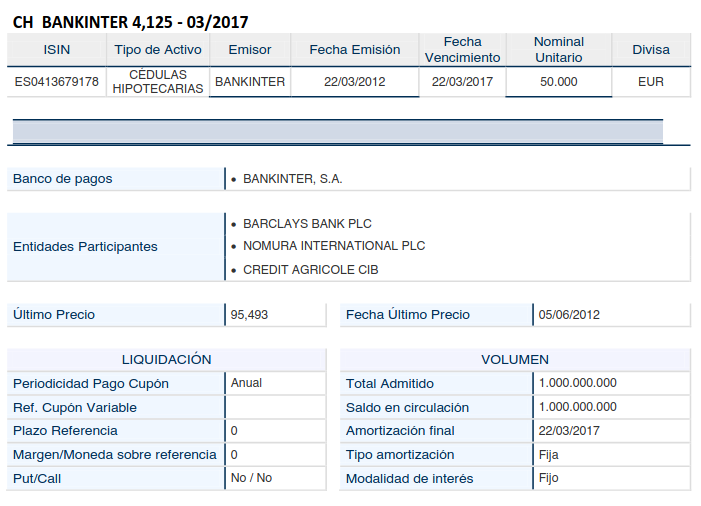
\includegraphics[width=0.9\textwidth]{../images/ej13.png}
    \caption{Cédulas Hipotecarias}
    \label{fig:cedulas}
\end{figure}

\begin{itemize}
    \item[a)] ¿Qué precio se pagó por cada Cédula Hipotecaria cuando se compró el 5/6/2012? \textbf{Sol: 48.170,30€}
    \item[b)] ¿Qué ecuación verifica la TIR con la que se contrataron estas Cédulas Hipotecarias el 5/6/2012? Comprueba que la TIR tiene un valor de 5,20\%.
    donde \(C\) es el cupón anual, \(F\) es el valor nominal, \(n\) es el número de años hasta el vencimiento, y \(TIR\) es la tasa interna de retorno.
    \item[c)] Sabiendo que el 5/6/2012 la duración de estas cédulas tenía un valor de 4,405537, ¿qué precio hubieran tenido las cédulas si la TIR se hubiera incrementado en 20 puntos básicos? \textbf{Sol: 47.766,87€} \textit{SIN RESOLVER}
\end{itemize}


\subsection*{Ejercicio 14}

La sociedad GADEB obtuvo financiación colocando en el mercado pagarés de empresa mediante una subasta competitiva. Estos pagarés tenían un nominal unitario de 6.000€ y vencimiento en 1 año. Después de anunciar la subasta en el mercado se recibieron las siguientes peticiones:

\begin{table}[H]
    \centering
    \begin{tabular}{|c|c|}
        \hline
        \textbf{Nominal (millones €)} & \textbf{Precio solicitado} \\ \hline
        20 & 95,975 \\ \hline
        30 & 95,885 \\ \hline
        35 & 94,975 \\ \hline
        25 & 94,555 \\ \hline
        10 & 94,375 \\ \hline
    \end{tabular}
\end{table}

Hoy, tres meses después de emitirse, estos pagarés se negocian en el mercado secundario mediante operaciones al contado al 4\% y también mediante operaciones con pacto de recompra a 15 días y al 3,5\%.

\begin{enumerate}[label=\textbf{\alph*)}]
    \item Resuelve la subasta sabiendo que la sociedad adjudicó un total de 100 millones y que para la adjudicación se usaron reglas similares a las aplicadas por el Tesoro Español. \textbf{Sol: medio: 95,385; marginal: 94,555}
    
    \item Calcula el tipo de interés marginal resultante de la subasta. \textbf{Sol: 5,7586\%}
    

    \item Si un inversor participó en la subasta solicitando pagarés a 94,975 y decide venderlos al contado hoy, ¿qué rentabilidad efectiva ha obtenido con ellos sabiendo que el intermediario en la operación de venta le cobra una comisión del 0,3\% sobre el efectivo de la venta? \textbf{Sol: 8\%}
    

    \item Calcula los precios que se fijan hoy en las operaciones con pacto de recompra y la rentabilidad efectiva que proporcionan este tipo de operaciones. \textbf{Sol: 5.846,53€; 5.855,05€; 3,6096\%}
    
\end{enumerate}





\subsection*{Ejercicio 15}

La empresa ALISUR posee en su cartera Letras del Tesoro por un nominal total de 60.000 euros. Estos valores fueron adquiridos en subasta al 7,75 \% de interés, con vencimiento a 92 días. Diez días después de la subasta la empresa debe realizar, en los 15 días posteriores, unos pagos por 39.290 euros, no disponiendo, en dicho momento, de liquidez para afrontarlos. El gerente de ALISUR decide solucionar el problema planteado a través de la venta de las letras, en la cantidad suficiente para hacer frente a los pagos. En estos momentos se puede conseguir para estos títulos un interés del 7,9335 \% en el mercado secundario. Una vez finalizado el período de pagos, la empresa volverá a adquirir las letras al 9,35 \% de interés. Los gastos totales de la operación de venta y compra se elevan al 2 por mil del nominal y se suponen pagaderos al final de la negociación simultánea.

Calcular el número de letras que debe vender ALISUR, el precio que habrá de pagar cuando decida comprarlas de nuevo y el coste que tiene asociado la operación de financiación diseñada. \textbf{Sol: 40 letras, 39.395,84€, 6,8\%}

\subsection*{Ejercicio 16}

El día 31/1/2017 un inversor contrató una operación simultánea sobre 100 obligaciones de la empresa ALALZA S.A. La operación simultánea estaba formada por las siguientes operaciones: compra al contado al 105,456 excupón y venta a plazo de 30 días (liquidación el 2/3/2017) al 4,504\% anual. Sabiendo que estas obligaciones tienen un nominal de 3.000€, pagan cupones anuales al 5\%, y vencen el 31/12/2030,

\begin{enumerate}
    \item[a)] ¿Cuánto pagó por cada obligación en la compra de la operación simultánea? \textbf{Sol: 3.176,42€}
    \item[b)] ¿Qué cantidad obtuvo por cada obligación en la venta de la operación simultánea? \textbf{Sol: 3.175,37€}
    \item[c)] Calcula la rentabilidad efectiva obtenida con esta operación simultánea \textbf{Sol: -0,40\%}
    \item[d)] En realidad, nuestro inversor esperaba, el 31/1/2017, que el precio de las obligaciones de la empresa ALALZA S.A. disminuyera en el mes siguiente; pensó que podría ser un buen negocio vender 100 obligaciones de esta clase para comprarlas 30 días después más baratas; y puesto que no disponía de dichas obligaciones, las adquirió temporalmente mediante la operación simultánea especificada en los apartados anteriores, para poder hacer la operación que había pensado. Si como había previsto nuestro inversor, el 2/3/2017 las obligaciones de ALALZA habían bajado de precio, cotizaban al 102,325 excupón. Calcula los beneficios o pérdidas que obtuvo nuestro inversor con la operación conjunta (operación simultánea + venta de las obligaciones el 31/1/17 y compra de las obligaciones el 2/3/2017). \textbf{Sol: 8.055,09€}
\end{enumerate}

\subsection*{Ejercicio 17}

Los fondos de inversión deben de tener una parte de su patrimonio invertida en activos muy líquidos para poder atender a los reembolsos de los partícipes; por ejemplo, en cuentas bancarias o en REPOS a un día. El 7/3/2017 los gestores del fondo INVERSIONES REUNIDAS contrataron una operación con pacto de recompra (REPO) sobre 1.500.000€ de nominal de Obligaciones del Estado con vencimiento el 31/1/2037 y cupón anual al 4,20\%. El REPO se contrató a 1 día y al -0,42\%. El precio de compra de las obligaciones al inicio del REPO (P1) se fijó como su precio de mercado con un recorte (haircut) del 5\%, de forma que P1=PMercado/(1+5\%). Sabiendo que el 7/3/2017 estas obligaciones cotizaban al 125,843 excupón, calcula:

\begin{enumerate}
    \item[a)] TIR con la que se estaban contratando las obligaciones en el mercado el 7/3/2017. \textbf{Sol: 2,529260\%}
    \item[b)] Cuantía pagada por el fondo al inicio de la operación REPO, 7/3/2017. \textbf{Sol: 1.803.510,57€}
    \item[c)] Cuantía que recibirá el fondo al final de la operación REPO, 8/3/2017. \textbf{Sol: 1.803.489,53€}
    \item[d)] ¿Cómo ha influido en la rentabilidad del fondo ésta operación? \textbf{Sol: Disminuye la rentabilidad}
\end{enumerate}


\chapter{Pasivos Financieros}

\section{Ejercicios Propuestos}

\subsection*{\textcolor{blue}{Ejercicio Propuesto 1}}

El 1 de mayo de 2019 la sociedad SABIOS, S.A. suscribe un préstamo de 50.000 € a un tipo de interés anual del 5\% a devolver en dos años con cuotas anuales constantes. La comisión de apertura ascendió a 600 € y los gastos de notaría a 500 €.

El cuadro de amortización facilitado por la entidad financiera en función del interés nominal del 5\% es el siguiente:

\begin{table}[H]
\centering
\begin{tabular}{|c|c|c|c|p{2cm}|}
\hline
\textbf{Vencimiento} & \textbf{Cuota} & \textbf{Capital} & \textbf{Intereses} & \textbf{Pendiente de Amortización} \\ \hline
01/05/2019 & - & - & - & 50.000 \\ \hline
01/05/2020 & 26.890 & 24.390 & 2.500 & 25.610 \\ \hline
01/05/2021 & 26.890 & 25.610 & 1.280 & 0 \\ \hline
\end{tabular}
\caption{CUADRO DE AMORTIZACIÓN A INTERÉS NOMINAL 5\%}
\end{table}

El cuadro de amortización obtenido mediante el criterio del tipo de interés efectivo del 6,5807\% responde al siguiente detalle:

\begin{table}[H]
\centering
\begin{tabular}{|c|c|c|c|c|}
\hline
\textbf{Vencimiento} & \textbf{Cuota} & \textbf{Capital} & \textbf{Intereses} & \textbf{Pendiente de Amortización} \\ \hline
01/05/2019 & - & - & - & 48.900 \\ \hline
01/05/2020 & 26.890 & 23.672 & 3.218 & 25.228 \\ \hline
01/05/2021 & 26.890 & 25.228 & 1.662 & 0 \\ \hline
\end{tabular}
\caption{CUADRO DE AMORTIZACIÓN A INTERÉS EFECTIVO 6,5807\%}
\end{table}

\textbf{SE PIDE:} Sabiendo que SABIOS, S.A. ha catalogado este pasivo en la categoría de Pasivos a coste amortizado, y empleando el sistema de capitalización compuesta, reflejo contable en el libro diario de las siguientes operaciones:
\begin{enumerate}[label=\alph*)]
\item Reconocimiento inicial por la obtención y cobro del préstamo.


\begin{table}[H]
    \centering
    \begin{tabular}{|p{2cm}|p{8cm}|p{2cm}|}
    \hline
    \rowcolor{blue!30}
    \textbf{DEBE} & \textbf{Reconcimiento inicial} & \textbf{HABER} \\
    \hline
    48.900&  \cuenta{572}& \\
    \hline
    &  5200. Préstamos a c/p con entidades de crédito& 23.672\\
    \hline
    &  170. Deudas a l/p con entidades de crédito& 25.228\\
    \hline
    \end{tabular}
\end{table}


\item Contabilización de los intereses devengados a 31/12/2019.

\begin{equation*}
    I_D = 48\p900 \times \left(1,065807^{8/12}\right) - 48\p900 = 2\p122,44
\end{equation*}


\begin{equation*}
    50\p000 \times \left(1,05^{8/12}\right) - 50\p000 = 1653,07
\end{equation*}

\begin{table}[H]
    \centering
    \begin{tabular}{|p{2cm}|p{8cm}|p{2cm}|}
    \hline
    \rowcolor{blue!30}
    \textbf{DEBE} & \textbf{Intereses a 31.12.19} & \textbf{HABER} \\
    \hline
    2.122,44&  6623. Intereses de deudas con entidades de crédito& \\
    \hline
    &  527. Intereses a c/p deudas con entidades de crédito& 1.653,07\\
    \hline
    &  5200. Préstamos a c/p con entidades de crédito& 469,37\\
    \hline
    \end{tabular}
\end{table}

\item Devengo y pago, en un único asiento, de la cuota correspondiente a 01/05/2020.

\begin{table}[H]
    \centering
    \begin{tabular}{|p{2cm}|p{8cm}|p{2cm}|}
    \hline
    \rowcolor{blue!30}
    \textbf{DEBE} & \textbf{Devengo y pago a 01.05.2020} & \textbf{HABER} \\
    \hline
    1.095,52&  6623. Intereses de deudas con entidades de crédito& \\
    \hline
    1.653,07& 527. Intereses a c/p de deudas con entidades de crédito & \\
    \hline
    24.141,37& 5200. Préstamos a c/p con entidades de crédito & \\
    \hline
    & \cuenta{572} & 26.890\\
    \hline
    \end{tabular}
\end{table}


\item Contabilice, exclusivamente, el pago de la cuota correspondiente a 01/05/2020.

\begin{table}[H]
    \centering
    \begin{tabular}{|p{2cm}|p{8cm}|p{2cm}|}
    \hline
    \rowcolor{blue!30}
    \textbf{DEBE} & \textbf{Pago cuota a 01.05.2020} & \textbf{HABER} \\
    \hline
    2.500 & 527. Intereses a c/p de deudas con entidades de crédito  & \\
    \hline
    24.390& 5200. Préstamos a c/p con entidades de crédito & \\
    \hline
    &  \cuenta{572}& 26.890\\
    \hline
    \end{tabular}
\end{table}


% \item Contabilización de los intereses devengados a 31/12/2020.


% \begin{table}[H]
%     \centering
%     \begin{tabular}{|p{2cm}|p{8cm}|p{2cm}|}
%     \hline
%     \rowcolor{blue!30}
%     \textbf{DEBE} & \textbf{Intereses a 31.12.2020} & \textbf{HABER} \\
%     \hline
%     &  & \\
%     \hline
%     &  & \\
%     \hline
%     &  & \\
%     \hline
%     &  & \\
%     \hline
%     \end{tabular}
% \end{table}

% \item Contabilice, exclusivamente, el devengo de intereses a 01/05/2021.


% \begin{table}[H]
%     \centering
%     \begin{tabular}{|p{2cm}|p{8cm}|p{2cm}|}
%     \hline
%     \rowcolor{blue!30}
%     \textbf{DEBE} & \textbf{} & \textbf{HABER} \\
%     \hline
%     &  & \\
%     \hline
%     &  & \\
%     \hline
%     &  & \\
%     \hline
%     &  & \\
%     \hline
%     \end{tabular}
%     \caption{Asiento X. Ejercicio X.}
%     \label{tabla:asientoXejXTx}
% \end{table}

% \item Contabilice, exclusivamente, el pago de la cuota a 01/05/2021.

% \begin{table}[H]
%     \centering
%     \begin{tabular}{|p{2cm}|p{8cm}|p{2cm}|}
%     \hline
%     \rowcolor{blue!30}
%     \textbf{DEBE} & \textbf{} & \textbf{HABER} \\
%     \hline
%     &  & \\
%     \hline
%     &  & \\
%     \hline
%     &  & \\
%     \hline
%     &  & \\
%     \hline
%     \end{tabular}
%     \caption{Asiento X. Ejercicio X.}
%     \label{tabla:asientoXejXTx}
% \end{table}

\begin{tcolorbox}[colframe=blue!30]
    Para más detalles, se encuentra ya hecho en el ejercicio 4 del apartado de ``Otros ejercicios'' en la página \pageref{sec:otros-ejercicios_ej4}.
\end{tcolorbox}

\end{enumerate}

\subsection*{\textcolor{blue}{Ejercicio Propuesto 2}}

La empresa CHA, S.A. realiza una emisión de deuda con las siguientes características: El 1 de marzo emite obligaciones no cotizadas a 3 años con un valor de emisión de 128.000 € y un valor de reembolso de 132.000 € (un valor nominal de 130.000 €). Los gastos de la operación ascienden a 1.000 € y el cupón anual es del 5\%. Tipo de interés efectivo es 6,3505\%. A continuación, se muestra el cuadro de amortización al tipo de interés efectivo y la valoración posterior a coste amortizado:

\begin{table}[h]
    \centering
    \begin{tabular}{|p{2cm}|p{2cm}|p{2cm}|p{2cm}|p{2cm}|p{2cm}|}
        \hline
        \textbf{Fecha} & \textbf{Cobro} & \textbf{Pagos} & \textbf{Intereses devengados (Gastos financieros)} & \textbf{Saldo amortizado} & \textbf{Coste Amortizado} \\
        \hline
        01/03/2023 & 127.000 &  &  &  & 127.000 \\
        \hline
        01/03/2024 &  & 6.500 & 8.065,16 & 1.565,16 & 128.565,17 \\
        \hline
        01/03/2025 &  & 6.500 & 8.164,56 & 1.664,56 & 130.229,73 \\
        \hline
        01/03/2026 &  & 138.500 & 8.270,27 & 130.229,73 & 0 \\
        \hline
    \end{tabular}
    \caption{Tabla de amortización}
    \label{tab:amortizacion}
\end{table}


\textbf{SE PIDE:} Registro contable de las siguientes operaciones:
\begin{enumerate}[label=\alph*)]
\item Emisión de la deuda a 01/03/2023.


\begin{table}[H]
    \centering
    \begin{tabular}{|p{2cm}|p{8cm}|p{2cm}|}
    \hline
    \rowcolor{blue!30}
    \textbf{DEBE} & \textbf{Emisión de deuda} & \textbf{HABER} \\
    \hline
    127.000& \cuenta{572} & \\
    \hline
    &  177. Obligaciones y bonos& 127.000\\
    \hline
    \end{tabular}
\end{table}


\item Si procede, devengo de intereses a 31/12/2023.

\begin{align*}
    I_T = \left[127\p000 \times 1,063505^{10/12}\right] - 127\p000 = 6.686,22 \\
    I_E = \left[130\p000 \times 1,05^{10/12}\right] - 130\p000 = 5\p394,52
\end{align*}
\begin{table}[H]
    \centering
    \begin{tabular}{|p{2cm}|p{8cm}|p{2cm}|}
    \hline
    \rowcolor{blue!30}
    \textbf{DEBE} & \textbf{Devengo de intereses 31.12.2023} & \textbf{HABER} \\
    \hline
    6.686,22& 6613. Intereses de obligaciones y bonos & \\
    \hline
    & 177. Obligaciones y bonos & 1291.70\\
    \hline
    &  506. Intereses de obligaciones y bonos a c/p& 5.394,52\\
    \hline
    \end{tabular}
\end{table}

\item Si procede, operaciones correspondientes al devengo y pago de los intereses explícitos a 01/03/2024.
\begin{align*}
    I_E = \left[(130\p000 + 5\p394,52) \times 1,05^{10/12}\right] - (130\p000 + 5\p394,52) = 1\p105,48 \\
\end{align*}

\begin{table}[H]
    \centering
    \begin{tabular}{|p{2cm}|p{8cm}|p{2cm}|}
    \hline
    \rowcolor{blue!30}
    \textbf{DEBE} & \textbf{Devengo de los intereses y pago de explícitos a 1.3.2024} & \textbf{HABER} \\
    \hline
    5.394,52& 506. Intereses de obligaciones y bonos & \\
    \hline
    1.105,48& 6613. Intereses de obligaciones y bonos & \\
    \hline
    &  \cuenta{572}& 6500\\
    \hline
    \end{tabular}
\end{table}


\item Si procede, en dos asientos, todas las operaciones correspondientes a 01/03/2025.

\begin{align*}
    I_T = \left[(128\p565,17 + 6\p768,63) \times 1,063505^{2/12} - \right] - (128\p565,17 + 6\p768,63) = 1\p395,90 \\
    I_E = \left[(130\p000+5\p394,52 \times 1,05^{2/12})\right]- (130\p000+5\p394,52) = 1\p105,48
\end{align*}

\begin{table}[H]
    \centering
    \begin{tabular}{|p{2cm}|p{8cm}|p{2cm}|}
    \hline
    \rowcolor{blue!30}
    \textbf{DEBE} & \textbf{Operaciones a 1.3.2025} & \textbf{HABER} \\
    \hline
     1.395,90&6613. Intereses de obligaciones y bonos &\\
    \hline
    &  177. Obligaciones y bonos& 290.48\\
    \hline
    & 506. Intereses de obligaciones y bonos & 1.105,48\\
    \hline
    &  SEGUNDO ASIENTO& \\
    \hline
    6.500&  506. Intereses de obligaciones y bonos & \\
    \hline
    &  \cuenta{572}&6.500 \\
    \hline
    \end{tabular}
\end{table}

\item Si procede, en un único asiento, todas las operaciones correspondientes a 01/03/2026.

\begin{align*}
    I_T = \left[(130\p229,73 + 6\p856,26) \times 1,063505^{2/12}\right] - (130\p229,73 + 6\p856,26) =  1\p413,97
\end{align*}
\begin{table}[H]
    \centering
    \begin{tabular}{|p{2cm}|p{8cm}|p{2cm}|}
    \hline
    \rowcolor{blue!30}
    \textbf{DEBE} & \textbf{Operaciones correspondientes a 1.3.2026} & \textbf{HABER} \\
    \hline
    5.394,52& 506. Intereses de obligaciones y bonos & \\
    \hline
    1.413,97&  6613. Intereses de obligaciones y bonos & \\
    \hline
    131.691,51& 500. Obligaciones y bonos a c/p & \\
    \hline
    &  \cuenta{572}& 138.500 \\
    \hline
    \end{tabular}
\end{table}

\end{enumerate}

\subsection*{\textcolor{blue}{Ejercicio Propuesto 3}}

El 1 de julio de 2021, la sociedad LUCERO, S.A. formaliza un préstamo con su banco por importe de 200.000 € a devolver durante los próximos 3 años. El interés nominal es de un 4,402\% anual, la comisión de estudios de un 2,5\% y la comisión de apertura del 1\%. El cuadro de amortización a interés nominal es el siguiente:

\begin{table}[H]
\centering
\begin{tabular}{|c|c|c|c|c|}
\hline
\textbf{Plazo} & \textbf{Cuota} & \textbf{Interés} & \textbf{Capital} & \textbf{Saldo pendiente de amortizar} \\ \hline
01/07/2021 & - & - & - & 200.000 \\ \hline
01/07/2022 & 72.620 & 8.804 & 63.816 & 136.184 \\ \hline
01/07/2023 & 72.620 & 5.994,82 & 66.625,18 & 69.558,82 \\ \hline
01/07/2024 & 72.620 & 3.061,18 & 69.558,82 & 0,00 \\ \hline
\end{tabular}
\caption{CUADRO DE AMORTIZACIÓN A INTERÉS NOMINAL 4,402\%}
\end{table}

El cuadro de amortización a un interés efectivo del 6,3117\% anual es el siguiente:

\begin{table}[H]
\centering
\begin{tabular}{|c|c|c|c|c|}
\hline
\textbf{Plazo} & \textbf{Cuota} & \textbf{Interés} & \textbf{Capital} & \textbf{Saldo pendiente de amortizar} \\ \hline
01/07/2021 & - & - & - & 193.000,00 \\ \hline
01/07/2022 & 72.620 & 12.181,58 & 60.438,42 & 132.561,58 \\ \hline
01/07/2023 & 72.620 & 8.366,89 & 64.253,11 & 68.308,47 \\ \hline
01/07/2024 & 72.620 & 4.311,53 & 68.308,47 & 0,00 \\ \hline
\end{tabular}
\caption{CUADRO DE AMORTIZACIÓN A INTERÉS EFECTIVO 6,3117\%}
\end{table}

Con fecha 01/07/2023, LUCERO, S.A. acuerda sustituir este préstamo por un pagaré con vencimiento a 3 años y un nominal de 70.000 € con un tipo de interés de mercado para esta operación del 10\%. El cuadro de amortización a coste amortizado del pagaré es el siguiente:

\begin{table}[H]
\centering
\begin{tabular}{|c|c|c|}
\hline
\textbf{Vencimientos} & \textbf{Cuota de interés} & \textbf{Saldo pendiente de amortizar} \\ \hline
01/07/2023 & - & 52.592,03 \\ \hline
01/07/2024 & 5.259,20 & 57.851,23 \\ \hline
01/07/2025 & 5.785,12 & 63.636,35 \\ \hline
01/07/2026 & 6.363,63 & 70.000 \\ \hline
\end{tabular}
\caption{CUADRO DE AMORTIZACIÓN DEL PAGARÉ}
\end{table}

\textbf{SE PIDE:} Realizar los asientos contables en el libro diario de la sociedad LUCERO, S.A. relativos a las siguientes operaciones:
\begin{enumerate}[label=\alph*)]
\item Reflejo contable del devengo de intereses y pago de la cuota a 01/07/2023 EN UN ÚNICO ASIENTO.

\begin{align*}
    \text{I. Totales}_{31/12/2022} = [132.561,58 \times (1,063117)^{6/12}] - 132.561,58 = 4.119,43 \, \text{€} \\
    \text{I. Explícitos}_{31/12/2022} = [136.184 \times (1,04402)^{6/12}] - 136.184 = 2.965,13 \, \text{€} \\
    \text{I. Implícitos}_{31/12/2022} = 4.119,43 - 2.965,13 = 1.154,30 \, \text{€} \\
    \text{I. Totales}_{01/07/2023} = \\ = [(132.561,58 + 4.119,43) \times (1,063117)^{6/12}] - (132.561,58 + 4.119,43) = 4.247,43 \, \text{€}
\end{align*}

\begin{table}[H]
    \centering
    \begin{tabular}{|p{2cm}|p{8cm}|p{2cm}|}
    \hline
    \rowcolor{blue!30}
    \textbf{DEBE} & \textbf{Devengo de intereses} & \textbf{HABER} \\
    \hline
    4.247,43&  662. Intereses de deudas& \\
    \hline
    1.965,13&  527. Intereses a c/p de deudas de entidades de crédito & \\
    \hline
   65.407,41 = 64.253,11 + 1.154,30 &  520 Deudas a c/p entidades d crédito& \\
    \hline
    &  \cuenta{572} & 72.620 \\
    \hline
    \end{tabular}
\end{table}


\item Realice los cálculos necesarios para determinar si las condiciones de los dos pasivos son o no sustancialmente diferentes a 01/07/2023.

\begin{align*}
    \text{Deuda antigua } = 68\p308,47 \\
    \frac{70\p000}{1,063117^3} = 58\p257,90 \rightarrow \text{Descontamos el valor nominal a 3 años} \\
    \text{Diferencia = } 68\p308,47 - 58\p257,90 = 10\p050,57\\
    10\% \times 68\p308,4 = 6\p830,84
\end{align*}
En base a los cálculos anteriores, podemos ver que \c{son sustancialmente diferentes, ya que la diferencia es mayor al 10\%}. Por lo tanto, debemos de da calcular la nueva deuda a su tipo de interés.

\begin{equation*}
    \frac{70\p000}{1,10^3} = 52\p592,03
\end{equation*}

% \begin{table}[H]
%     \centering
%     \begin{tabular}{|p{2cm}|p{8cm}|p{2cm}|}
%     \hline
%     \rowcolor{blue!30}
%     \textbf{DEBE} & \textbf{} & \textbf{HABER} \\
%     \hline
%     &  & \\
%     \hline
%     &  & \\
%     \hline
%     &  & \\
%     \hline
%     &  & \\
%     \hline
%     \end{tabular}
% \end{table}


\item Reflejo contable del cambio del endeudamiento a 01/07/2023 en base a la conclusión obtenida en el apartado anterior.

\begin{table}[H]
    \centering
    \begin{tabular}{|p{2cm}|p{8cm}|p{2cm}|}
    \hline
    \rowcolor{blue!30}
    \textbf{DEBE} & \textbf{Cambio del endeudamiento a 1.7.2023} & \textbf{HABER} \\
    \hline
    68\p308,4&  170. Deudas a l/p con Entidades de crédito& \\
    \hline
    & 170. Deudas a l/p con Entidades de crédito&52.592,03 \\
    \hline
    &  7691. Otros ingresos derivados del intercambio de cuentas& 15.716,44\\
    \hline
    \end{tabular}
\end{table}


\item Reflejo contable del pago de la cuota a 01/07/2025.
\begin{table}[H]
    \centering
    \begin{tabular}{|p{2cm}|p{8cm}|p{2cm}|}
    \hline
    \rowcolor{blue!30}
    \textbf{DEBE} & \textbf{Pago de la cuota a 01/07/2025} & \textbf{HABER} \\
    \hline
    & NO PROCEDE ASIENTO CONTABLE  &\\
    \hline
    \end{tabular}
\end{table}

\end{enumerate}






\section{Otros Ejercicios}

\subsection*{\textcolor{red}{Ejercicio 1}}

La empresa COPA, S.A. recibe un préstamo por un valor nominal de 50.000 € el día 1 de enero de 2019 con un vencimiento a tres años y un valor de reembolso de 52.000 €, al tipo de interés nominal del 5\%. Los gastos de la operación (que corren a cargo de la empresa COPA) ascienden a 1.000 €. El tipo de interés efectivo de la operación es del 7,006\%. El cuadro de amortización calculado en base al tipo de interés efectivo es el siguiente:

\begin{table}[h!]
\centering
\begin{tabular}{|p{2cm}|p{3cm}|p{2cm}|p{3cm}|p{3cm}|}
\hline
\textbf{Plazo} & \textbf{Intereses Devengados} & \textbf{Pagos} & \textbf{Saldo amortizado} & \textbf{Saldo pendiente de amortizar} \\ \hline
01/01/2019 & - & - & - & 50.000 \\ \hline
31/12/2019 & 3.433 & 2.500 & 933 & 49.933 \\ \hline
31/12/2020 & 3.498 & 2.500 & 998 & 50.932 \\ \hline
31/12/2021 & 3.563 & 52.500 & 50.932 & 0 \\ \hline
\end{tabular}
\caption{CUADRO DE AMORTIZACIÓN A COSTE EFECTIVO 7,006\%}
\end{table}

\textbf{SE PIDE:} contabilizar las siguientes operaciones:
\begin{enumerate}[label=\alph*)]


\item Obtención del préstamo a 01/01/2019.

\begin{table}[H]
\centering
\begin{tabular}{|p{2cm}|p{8cm}|p{2cm}|}
\hline
\rowcolor{blue!30}
\textbf{DEBE} & \textbf{Obtención del préstamo el 01/01/2019} & \textbf{HABER} \\ \hline
49.000 & (572) Bancos c/c & \\ \hline
& (170) Deudas a largo plazo con entidades de crédito & 49.000 \\ \hline
\end{tabular}
\end{table}

\item Contabilización de las operaciones necesarias a 31/12/2019.

\begin{table}[H]
\centering
\begin{tabular}{|p{2cm}|p{8cm}|p{2cm}|}
\hline
\rowcolor{blue!30}
\textbf{DEBE} & \textbf{Contabilización de las operaciones necesarias a 31/12/2019} & \textbf{HABER} \\ \hline
3.433 & (662) Intereses de deudas & \\ \hline
& (170) Deudas a l/p con entidades de crédito & 933 \\ \hline
& (572) Bancos c/c & 2.500 \\ \hline
\end{tabular}
\end{table}

\item Contabilización de la reclasificación de la deuda a 31/12/2020.

No es necesario, pero debemos de tener de asumir que antes de reclasificar la deuda a largo plazo, se han contabilizado los interses devengados y pagados.

\begin{table}[H]
\centering
\begin{tabular}{|p{2cm}|p{8cm}|p{2cm}|}
\hline
\rowcolor{blue!30}
\textbf{DEBE} & \textbf{Devengo de intereses a 31/12/2020} & \textbf{HABER} \\ \hline
3.498 & (662) Intereses de deudas & \\ \hline
& (170) Deudas a l/p con entidades de crédito & 998 \\ \hline
& (572) Bancos c/c & 2.500 \\ \hline
\end{tabular}
\end{table}

Una vez contabilizados los intereses devengados y pagados, se procede a reclasificar la deuda a largo plazo a corto plazo.

\begin{table}[H]
\centering
\begin{tabular}{|p{2cm}|p{8cm}|p{2cm}|}
\hline
\rowcolor{blue!30}
\textbf{DEBE} & \textbf{Contabilización de la reclasificación de la deuda a 31/12/2020} & \textbf{HABER} \\ \hline
50.932 & (170) Deudas largo plazo entidades crédito & \\ \hline
& (520) Deudas a corto plazo entidades crédito & 50.932 \\ \hline
\end{tabular}
\end{table}
\item Contabilización de la cancelación de la deuda EXCLUSIVAMENTE por su valor de reembolso el 31/12/2021.
\begin{table}[H]
\centering
\begin{tabular}{|p{2cm}|p{8cm}|p{2cm}|}
\hline
\rowcolor{blue!30}
\textbf{DEBE} & \textbf{Contabilización de la cancelación de la deuda EXCLUSIVAMENTE por su valor de reembolso el 31/12/2021} & \textbf{HABER} \\ \hline
52.000 & (520) Deudas a corto plazo con entidades de crédito & \\ \hline
& (572) Bancos c/c & 52.000 \\ \hline
\end{tabular}
\end{table}

\end{enumerate}


\newpage
\subsection*{\textcolor{red}{Ejercicio 2}}

La empresa TUNA, S.A. concede el 1 de enero de 2018 un préstamo de 10.000 € a la empresa VELVAT S.A, a devolver en 3 años en cuotas constantes anuales y cuyo cuadro de amortización según el tipo de interés efectivo al 7\% es el siguiente:

\begin{table}[h!]
\centering
\begin{tabular}{|c|c|c|c|c|c|}
\hline
\textbf{Fecha} & \textbf{Cobro} & \textbf{Pagos (cuota)} & \textbf{Intereses} & \textbf{Capital} & \textbf{Coste amortizado} \\ \hline
01/01/2018 & 10.000 & - & - & - & 10.000 \\ \hline
31/12/2018 & - & 3.810,52 & 700 & 3.110,52 & 6.889,48 \\ \hline
31/12/2019 & - & 3.810,52 & 482,26 & 3.328,25 & 3.561,23 \\ \hline
31/12/2020 & - & 3.810,52 & 249,29 & 3.561,23 & 0 \\ \hline
\end{tabular}
\caption{CUADRO DE AMORTIZACIÓN A COSTE EFECTIVO 7\%}
\end{table}

\textbf{SE PIDE:} contabilizar los siguientes apartados para la empresa VELVAT, S.A.:
\begin{enumerate}[label=\alph*)]
\item Asiento contable de la formalización del préstamo el 01/01/2018.

\begin{table}[H]
\centering
\begin{tabular}{|p{2cm}|p{8cm}|p{2cm}|}
\hline
\rowcolor{blue!30}
\textbf{DEBE} & \textbf{Asiento contable de la formalización del préstamo el 01/01/2018} & \textbf{HABER} \\ \hline
10.000 & (572) Bancos c/c & \\ \hline
& (520) Deudas a corto plazo con entidades de crédito & 3.110,52 \\ \hline
& (170) Deudas a largo plazo con entidades de crédito & 6.889,48 \\ \hline
\end{tabular}
\end{table}

\item Asiento contable del pago de la primera cuota el 31/12/2018.

\begin{table}[H]
\centering
\begin{tabular}{|p{2cm}|p{8cm}|p{2cm}|}
\hline
\rowcolor{blue!30}
\textbf{DEBE} & \textbf{Asiento contable del pago de la primera cuota el 31/12/2018} & \textbf{HABER} \\ \hline
3.110,52 & (520) Deudas a corto plazo con entidades de crédito & \\ \hline
700 & (662) Intereses de deudas & \\ \hline
& (572) Bancos c/c & 3.810,52 \\ \hline
\end{tabular}
\end{table}

\item Asiento contable de la reclasificación de la obligación de pago el 31/12/2019.

\begin{table}[H]
\centering
\begin{tabular}{|p{2cm}|p{8cm}|p{2cm}|}
\hline
\rowcolor{blue!30}
\textbf{DEBE} & \textbf{Asiento contable de la reclasificación de la obligación de pago el 31/12/2019} & \textbf{HABER} \\ \hline
3.561,23 & (170) Deudas a largo plazo con entidades de crédito & \\ \hline
& (520) Deudas a corto plazo con entidades de crédito & 3.561,23 \\ \hline
\end{tabular}
\end{table}

\item Asiento contable del pago de la última cuota el 31/12/2020.
\end{enumerate}

\begin{table}[H]
\centering
\begin{tabular}{|p{2cm}|p{8cm}|p{2cm}|}
\hline
\rowcolor{blue!30}
\textbf{DEBE} & \textbf{Asiento contable del pago de la última cuota el 31/12/2020} & \textbf{HABER} \\ \hline
3.561,23 & (520) Deudas a corto plazo con entidades de crédito & \\ \hline
249,29 & (662) Intereses de deudas & \\ \hline
& (572) Bancos c/c & 3.810,52 \\ \hline
\end{tabular}
\end{table}

\newpage
\subsection*{\textcolor{red}{Ejercicio 3}}

La empresa CONFINADOS, S.A. realiza una emisión de 1.000 obligaciones el 1 de julio de 2019, cobrando por ellas un total de 130.000 €. Su vencimiento, que es único, tendrá lugar el 30 de junio del año 2021, con un valor de reembolso total de 150.000 €. El nominal de las obligaciones es de 150 € cada una.

La tabla, que recoge el coste amortizado al tipo de interés efectivo del 7,417231\%, es la siguiente:

\begin{table}[h]
    \centering
    \renewcommand{\arraystretch}{1.2}
    \begin{tabular}{|c|r|r|p{2cm}|p{2cm}|p{2cm}|}
        \hline
        \textbf{Fecha} & \textbf{Cobro} & \textbf{Pagos} & \textbf{Intereses devengados} & \textbf{Saldo amortizado} & \textbf{Saldo pendiente de amortizar} \\
        \hline
        01/07/2019 & 130.000 & 0 &  &  & 130.000 \\
        31/12/2019 & 0 & 0 & 4.734,97 & 4.734,97 & 134.734,97 \\
        31/12/2020 & 0 & 0 & 9.993,60 & 9.993,60 & 144.728,57 \\
        01/07/2021 & 150.000 & 0 & 5.271,43 & 144.728,57 & 0 \\
        \hline
    \end{tabular}
    \caption{Tabla de amortización}
    \label{tab:amortizacion}
\end{table}


\textbf{SE PIDE:} Realizar los asientos contables en el libro diario de la sociedad CONFINADOS S.A. relativos a las siguientes operaciones:
\begin{enumerate}[label=\alph*)]
\item Contabilización, el 01/07/2019, de la emisión de la deuda.

\begin{table}[H]
\centering
\begin{tabular}{|p{2cm}|p{8cm}|p{2cm}|}
\hline
\rowcolor{blue!30}
\textbf{DEBE} & \textbf{Contabilización, el 01/07/2019, de la emisión de la deuda} & \textbf{HABER} \\ \hline
130.000 & (572) Bancos c/c & \\ \hline
& (177) Obligaciones y bonos & 130.000 \\ \hline
\end{tabular}
\end{table}

\item Contabilización, si procede, del devengo de intereses explícitos e implícitos a 31/12/2019.

En este caso cabe destacar que como durante ``vida'' de la deuda no se efectúa ningún pago, no van a existir intereses explícitos, por lo que los consideramos en su totalidad \c{implícitos}.

\begin{table}[H]
\centering
\begin{tabular}{|p{2cm}|p{8cm}|p{2cm}|}
\hline
\rowcolor{blue!30}
\textbf{DEBE} & \textbf{Contabilización, si procede, del devengo de intereses explícitos e implícitos a 31/12/2019} & \textbf{HABER} \\ \hline
4.734,97 & (661) Intereses de obligaciones y bonos & \\ \hline
& (177) Obligaciones y bonos & 4.734,97 \\ \hline
\end{tabular}
\end{table}

\item Contabilización, si procede, del pago de intereses explícitos a 31/12/2019.

\begin{table}[H]
\centering
\begin{tabular}{|p{2cm}|p{8cm}|p{2cm}|}
\hline
\rowcolor{blue!30}
\textbf{DEBE} & \textbf{Contabilización, si procede, del pago de intereses explícitos a 31/12/2019} & \textbf{HABER} \\ \hline
\multicolumn{3}{|c|}{NO PROCEDE ANOTACIÓN CONTABLE} \\ \hline
\end{tabular}
\end{table}

\item Asientos a realizar por la empresa CONFINADOS S.A., en su caso, a 31/12/2020.

Deberán de realizar dos anotaciones contables:
\begin{enumerate}
    \item Registrar los intereses devengados durante el año 2020.
    \item Reclasificar la deuda a largo plazo a corto plazo.
\end{enumerate}

\begin{table}[H]
\centering
\begin{tabular}{|p{2cm}|p{8cm}|p{2cm}|}
\hline
\rowcolor{blue!30}
\textbf{DEBE} & \textbf{Registrar los intereses devengados durante el año 2020} & \textbf{HABER} \\ \hline
9.993,6 & (661) Intereses de obligaciones y bonos & \\ \hline
& (177) Obligaciones y bonos & 9.993,6 \\ \hline
\end{tabular}
\end{table}

\begin{table}[H]
\centering
\begin{tabular}{|p{2cm}|p{8cm}|p{2cm}|}
\hline
\rowcolor{blue!30}
\textbf{DEBE} & \textbf{Reclasificar la deuda a largo plazo a corto plazo} & \textbf{HABER} \\ \hline
144.728,57 & (177) Obligaciones y bonos & \\ \hline
& (500) Obligaciones y bonos a corto plazo & 144.728,57 \\ \hline
\end{tabular}
\end{table}

\c{Se puede hacer en un solo asiento, pero se ha desglosado para una mejor comprensión.}

\item Contabilización, si procede, en un solo asiento, de los intereses devengados y reembolso del principal a 01/07/2021.

\begin{table}[H]
\centering
\begin{tabular}{|p{2cm}|p{8cm}|p{2cm}|}
\hline
\rowcolor{blue!30}
\textbf{DEBE} & \textbf{Contabilización, si procede, en un solo asiento, de los intereses devengados y reembolso del principal a 01/07/2021} & \textbf{HABER} \\ \hline
5.271,38 & (661) Intereses de obligaciones y bonos & \\ \hline
144.728,6 & (500) Obligaciones y bonos a corto plazo & \\ \hline
& (572) Bancos c/c & 150.000 \\ \hline
\end{tabular}
\end{table}

\end{enumerate}


\newpage
\subsection*{\textcolor{red}{Ejercicio 4}} \label{sec:otros-ejercicios_ej4}

La empresa SABIOS, S.A. suscribe un préstamo de 50.000 € a un tipo de interés anual del 5\% a devolver en dos años con cuotas anuales constantes. La comisión de apertura ascendió a 600 € y los gastos de notaría a 500 €.

El cuadro de amortización facilitado por la entidad financiera en función del interés nominal del 5\% es el siguiente:

\begin{table}[H]
\centering
\begin{tabular}{|c|c|c|c|c|}
\hline
\textbf{Vencimiento} & \textbf{Cuota} & \textbf{Capital} & \textbf{Intereses} & \textbf{Pendiente de Amortización} \\ \hline
01/05/2019 & - & - & - & 50.000 \\ \hline
01/05/2020 & 26.890 & 24.390 & 2.500 & 25.610 \\ \hline
01/05/2021 & 26.890 & 25.610 & 1.280 & 0 \\ \hline
\end{tabular}
\caption{CUADRO DE AMORTIZACIÓN A INTERÉS NOMINAL 5\%}
\end{table}

El cuadro de amortización obtenido mediante el criterio del tipo de interés efectivo del 6,5807\% responde al siguiente detalle:

\begin{table}[h!]
\centering
\begin{tabular}{|c|c|c|c|c|}
\hline
\textbf{Vencimiento} & \textbf{Cuota} & \textbf{Capital} & \textbf{Intereses} & \textbf{Pendiente de Amortización} \\ \hline
01/05/2019 & - & - & - & 48.900 \\ \hline
01/05/2020 & 26.890 & 23.672 & 3.218 & 25.228 \\ \hline
01/05/2021 & 26.890 & 25.228 & 1.662 & 0 \\ \hline
\end{tabular}
\caption{CUADRO DE AMORTIZACIÓN A INTERÉS EFECTIVO 6,5807\%}
\end{table}

\textbf{SE PIDE:} Sabiendo que SABIOS, S.A. ha catalogado este pasivo en la categoría de Préstamos y partidas a pagar, y empleando el sistema de capitalización compuesta, reflejo contable en el libro diario de las siguientes operaciones:
\begin{enumerate}[label=\alph*)]
\item Reconocimiento inicial por la obtención y cobro del préstamo.

\begin{table}[H]
\centering
\begin{tabular}{|p{2cm}|p{8cm}|p{2cm}|}
\hline
\rowcolor{blue!30}
\textbf{DEBE} & \textbf{Reconocimiento inicial por la obtención y cobro del préstamo} & \textbf{HABER} \\ \hline
48.900 & (572) Bancos c/c & \\ \hline
& (5200) Préstamos a c/p con entidades de crédito & 23.672 \\ \hline
& (170) Deudas a l/p con entidades de crédito & 25.228 \\ \hline
\end{tabular}
\end{table}

\item Contabilización de los intereses devengados a 31/12/2019.

Por un lado, debemos de calcular los intereses totales que se han devengado durante 8 meses que podemos ver en la figura \ref{fig:intereses_devengados_ejercicio4}.

\begin{figure}[H]
    \begin{equation*}
        \text{Intereses totales}  = \left[48\p900 \times (1,0658 / 12 )\right] - 48\p900 = 2\p122,44 \text{ €}
    \end{equation*}
    \caption{Cálculo de los intereses devengados a 31/12/2019.}
    \label{fig:intereses_devengados_ejercicio4}
\end{figure} 

Ahora debemos de calcualar los intereses explícitos que podemos ver en la figura \ref{fig:intereses_explicitos_ejercicio4}, así como los intereses implícitos que podemos ver en la figura \ref{fig:intereses_implicitos_ejercicio4}.
\begin{figure}[H]
    \begin{equation*}
        \text{Intereses explícitos} = 50\p000 \times (1,058 / 12) - 50\p000 = 1\p653,07 \text{ €}
    \end{equation*}
    \caption{Cálculo de los intereses explícitos a 31/12/2019.}
    \label{fig:intereses_explicitos_ejercicio4}
\end{figure}

\begin{figure}[H]
    \begin{equation*}
        \text{Intereses implícitos} = 2\p122,44 - 1\p653,07 = 471,38 \text{ €}
    \end{equation*}
    \caption{Cálculo de los intereses implícitos a 31/12/2019.}
    \label{fig:intereses_implicitos_ejercicio4}
\end{figure}


\begin{table}[H]
\centering
\begin{tabular}{|p{2cm}|p{8cm}|p{2cm}|}
\hline
\rowcolor{blue!30}
\textbf{DEBE} & \textbf{Contabilización de los intereses devengados a 31/12/2019} & \textbf{HABER} \\ \hline
2.122,44 & (6623) Intereses de deudas con entidades de crédito & \\ \hline
& (527) Intereses a c/p deudas con entidades de crédito & 1.653,07 \\ \hline
& (5200) Préstamos a c/p con entidades de crédito & 469,37 \\ \hline
\end{tabular}
\end{table}

\item Devengo y pago, en un único asiento, de la cuota correspondiente a 01/05/2020.

\begin{align*}
    \text{Intereses totales} = \\
    \\ = \left[\left(48\p900+2\p122,44\right) \times \left(1,065807/12\right)\right] - \left(48\p900+2\p122,44\right) = 1\p095,52 \text{ €}
\end{align*}

\begin{table}[H]
\centering
\begin{tabular}{|p{2cm}|p{8cm}|p{2cm}|}
\hline
\rowcolor{blue!30}
\textbf{DEBE} & \textbf{Devengo y pago, en un único asiento, de la cuota correspondiente a 01/05/2020} & \textbf{HABER} \\ \hline
1.095,52 & (6623) Intereses de deudas a c/p con entidades de crédito & \\ \hline
1.653,07 & (527) Intereses a c/p de deudas con entidades de crédito & \\ \hline
24.141,37 & (5200) Préstamos a c/p con entidades de crédito & \\ \hline
& (572) Bancos c/c & 26.890 \\ \hline
\end{tabular}
\end{table}


\item Contabilice, exclusivamente, el pago de la cuota correspondiente a 01/05/2020.

\begin{table}[H]
\centering
\begin{tabular}{|p{2cm}|p{8cm}|p{2cm}|}
\hline
\rowcolor{blue!30}
\textbf{DEBE} & \textbf{Contabilice, exclusivamente, el pago de la cuota correspondiente a 01/05/2020} & \textbf{HABER} \\ \hline
2.500 & (527) Intereses a c/p de deudas con entidades de crédito & \\ \hline
24.390 & (5200) Préstamos a c/p con entidades de crédito & \\ \hline
& (572) Bancos c/c & 26.890 \\ \hline
\end{tabular}
\end{table}

\item Contabilice, exclusivamente, los intereses devengados a 31/12/2020.

\begin{figure}[H]
    \begin{align*}
        \text{Intereses totales} &= \left[25.228 \times \left(1,065807^{8/12}\right)\right] - 25.228 = 1.094,98 \text{ €} \\
        \text{Intereses explícitos} &= \left[25.609 \times \left(1,05^{8/12}\right)\right] - 25.609 = 846,67 \text{ €} \\
        \text{Intereses implícitos} &= 1.094,98 - 846,67 = 248,31 \text{ €}
    \end{align*}
    \caption{Cálculo de los intereses devengados a 31/12/2020.}
    \label{fig:intereses_devengados_ejercicio4_2020}
\end{figure}

\begin{table}[H]
\centering
\begin{tabular}{|p{2cm}|p{8cm}|p{2cm}|}
\hline
\rowcolor{blue!30}
\textbf{DEBE} & \textbf{Contabilice, exclusivamente, los intereses devengados a 31/12/2020} & \textbf{HABER} \\ \hline
1.094,98 & (6623) Intereses de deudas con entidades de crédito & \\ \hline
& (527) Intereses a c/p deudas con entidades de crédito & 846,67 \\ \hline
& (5200) Préstamos a c/p con entidades de crédito & 248,31 \\ \hline
\end{tabular}
\end{table}

\item Contabilice, exclusivamente, el devengo de los intereses a 01/05/2021.

\begin{figure}[H]
    \begin{align*}
        \text{Intereses totales} &= \left[\left(25.228 + 1.094,98\right) \times \left(1,065807^{4/12}\right)\right] - \left(25.228 + 1.094,98\right) = 565,19 \text{ €} \\
        \text{Intereses explícitos} &= \left[\left(25.610 + 846,67\right) \times \left(1,05^{4/12}\right)\right] - \left(25.610 + 846,67\right) = 433,80 \text{ €} \\
        \text{Intereses implícitos} &= 565,19 - 433,80 = 131,39 \text{ €}
    \end{align*}
    \caption{Cálculo de los intereses devengados a 01/05/2021.}
    \label{fig:intereses_devengados_ejercicio4_2021}
\end{figure}

\begin{table}[H]
\centering
\begin{tabular}{|p{2cm}|p{8cm}|p{2cm}|}
\hline
\rowcolor{blue!30}
\textbf{DEBE} & \textbf{Contabilice, exclusivamente, el devengo de los intereses a 01/05/2021} & \textbf{HABER} \\ \hline
565,19 & (6623) Intereses de deudas a c/p con entidades de crédito & \\ \hline
& (527) Intereses a c/p deudas con entidades de crédito & 433,80 \\ \hline
& (5200) Préstamos a c/p con entidades de crédito & 131,39 \\ \hline
\end{tabular}
\end{table}

\item Contabilice, exclusivamente, el pago de la cuota a 01/05/2021.

\begin{table}[H]
\centering
\begin{tabular}{|p{2cm}|p{8cm}|p{2cm}|}
\hline
\rowcolor{blue!30}
\textbf{DEBE} & \textbf{Contabilice, exclusivamente, el pago de la cuota a 01/05/2021} & \textbf{HABER} \\ \hline
1.280 & (527) Intereses a c/p de deudas con entidades de crédito & \\ \hline
25.610 & (5200) Préstamos a c/p con entidades de crédito & \\ \hline
& (572) Bancos c/c & 26.890 \\ \hline
\end{tabular}
\end{table}

\end{enumerate}



\chapter{Fondos Propios}
\includepdf[pages=2-]{EjerciciosMD/PropuestosT4}

\chapter{Provisiones y Contingencias}
\includepdf[pages=2-]{EjerciciosMD/PropuestosT5}

\chapter{Impuesto sobre beneficios}
\includepdf[pages=2-]{EjerciciosMD/PropuestosT6}

%\chapter{Fondos Propios}
%\documentclass[a4paper,12pt]{article}

% Paquetes básicos
\usepackage[utf8]{inputenc}
\usepackage[T1]{fontenc}
\usepackage[spanish]{babel}
\usepackage{graphicx}
\usepackage{xcolor}
\usepackage{lipsum}
\usepackage{geometry}
\geometry{top=3cm, bottom=3cm, left=2.5cm, right=2.5cm}

% Paquetes para diseño
\usepackage{titlesec}
\usepackage{fancyhdr}
\usepackage{amsmath}
\usepackage{textgreek}
\usepackage{amssymb}
\usepackage{hyperref}

% Paquetes para el entorno lstlisting
\usepackage{listings}
\usepackage{inconsolata}

%encabezado y pie de página nivel profesional
\usepackage{fancyhdr}
\pagestyle{fancy}
\fancyhf{}
\fancyhead[L]{\leftmark}
\fancyhead[R]{\rightmark}
\fancyfoot[L]{\textbf{Ismael Sallami Moreno - GIIADE}}
\fancyfoot[C]{\thepage}
\fancyfoot[R]{\textbf{(UGR)} \today}
\renewcommand{\headrulewidth}{0.4pt}
\renewcommand{\footrulewidth}{0.4pt}
\setlength{\headheight}{15pt}
\setlength{\headsep}{10pt}
\setlength{\footskip}{20pt}
\usepackage{truncate}
\fancyhead[L]{\truncate{0.5\headwidth}{\leftmark}}
\fancyhead[R]{\truncate{0.5\headwidth}{\rightmark}}
\usepackage{mathpazo}
\usepackage{tcolorbox}
\usepackage{array}



% Paquete para fondo
\usepackage{background}
\usepackage{float}

% Configuración de lstlisting
\lstset{
    inputencoding=utf8,          % Permite UTF-8
    extendedchars=true,          % Reconoce caracteres extendidos
    literate=                    % Configuración manual para tildes y símbolos
        {á}{{\'a}}1
        {é}{{\'e}}1
        {í}{{\'i}}1
        {ó}{{\'o}}1
        {ú}{{\'u}}1
        {ñ}{{\~n}}1
        {Á}{{\'A}}1
        {É}{{\'E}}1
        {Í}{{\'I}}1
        {Ó}{{\'O}}1
        {Ú}{{\'U}}1
        {Ñ}{{\~N}}1
        {¿}{{\textquestiondown}}1
        {¡}{{\textexclamdown}}1,
    basicstyle=\ttfamily,        % Fuente monoespaciada
    breaklines=true,             % Habilita salto de línea automático
    frame=single,                % Marco alrededor del código
    backgroundcolor=\color{gray!10}, % Fondo gris claro
    keywordstyle=\color{blue},   % Color para palabras clave
    commentstyle=\color{green},  % Color para comentarios
    stringstyle=\color{red}      % Color para strings
}
\lstdefinestyle{customcpp}{
    language=C++,                % Lenguaje de programación
    showspaces=false,            % No mostrar espacios
    showtabs=false,              % No mostrar tabulaciones
    tabsize=4,                   % Tamaño de tabulación
    showstringspaces=false,      % No mostrar espacios en strings
    numbers=left,                % Números de línea a la izquierda
    numberstyle=\tiny\color{gray}, % Estilo de los números de línea
    numbersep=5pt,               % Separación de los números de línea
    stepnumber=1,                % Mostrar número en cada línea
    basicstyle=\ttfamily\footnotesize, % Estilo básico del código
    keywordstyle=\bfseries\color{blue}, % Estilo de las palabras clave
    commentstyle=\itshape\color{green!50!black}, % Estilo de los comentarios
    stringstyle=\color{red},     % Estilo de los strings
    identifierstyle=\color{black}, % Estilo de los identificadores
    % procnamekeys={def,class},    % Palabras clave para nombres de funciones
    morekeywords={constexpr,nullptr,size_t}, % Más palabras clave
    emph={int,char,double,float,unsigned}, % Palabras a enfatizar
    emphstyle=\color{magenta},   % Estilo de las palabras enfatizadas
    backgroundcolor=\color{gray!10}, % Color de fondo
    frame=shadowbox,             % Marco con sombra
    rulesepcolor=\color{gray},   % Color de la línea de separación
    breakatwhitespace=false,     % No cortar en espacios en blanco
    breaklines=true,             % Cortar líneas largas
    captionpos=b,                % Posición del título (abajo)
    escapeinside={(*@}{@*)},     % Delimitadores para escapar a LaTeX
    morecomment=[l][\color{magenta}]{\#}, % Comentarios de una línea
    morecomment=[s][\color{orange}]{/*}{*/}, % Comentarios multilínea
    morestring=[b],             % Strings entre comillas dobles
    morestring=[b]'              % Strings entre comillas simples
}

% Configuración de título
\titleformat{\section}{\normalfont\Large\bfseries}{\thesection}{1em}{}

% Información del documento
\title{
    \vspace{-2cm}
    
\includegraphics[width=0.3\textwidth]{images/etsiit.png} \\ % Cambia el logo si es necesario
    \LARGE Ingeniería Informática + ADE\\
    \large Universidad de Granada (UGR)\\[1cm]
}
\author{\textbf{Autor:} Ismael Sallami Moreno}
\date{\textbf{Asignatura:} Tema 4: Seguridad en Redes (FR)\\[1cm]}

% Configuración del fondo
\backgroundsetup{
    scale=1,
    color=black,
    opacity=0.2,
    angle=0,
    position=current page.south,
    vshift=0pt,
    hshift=0pt,
    contents={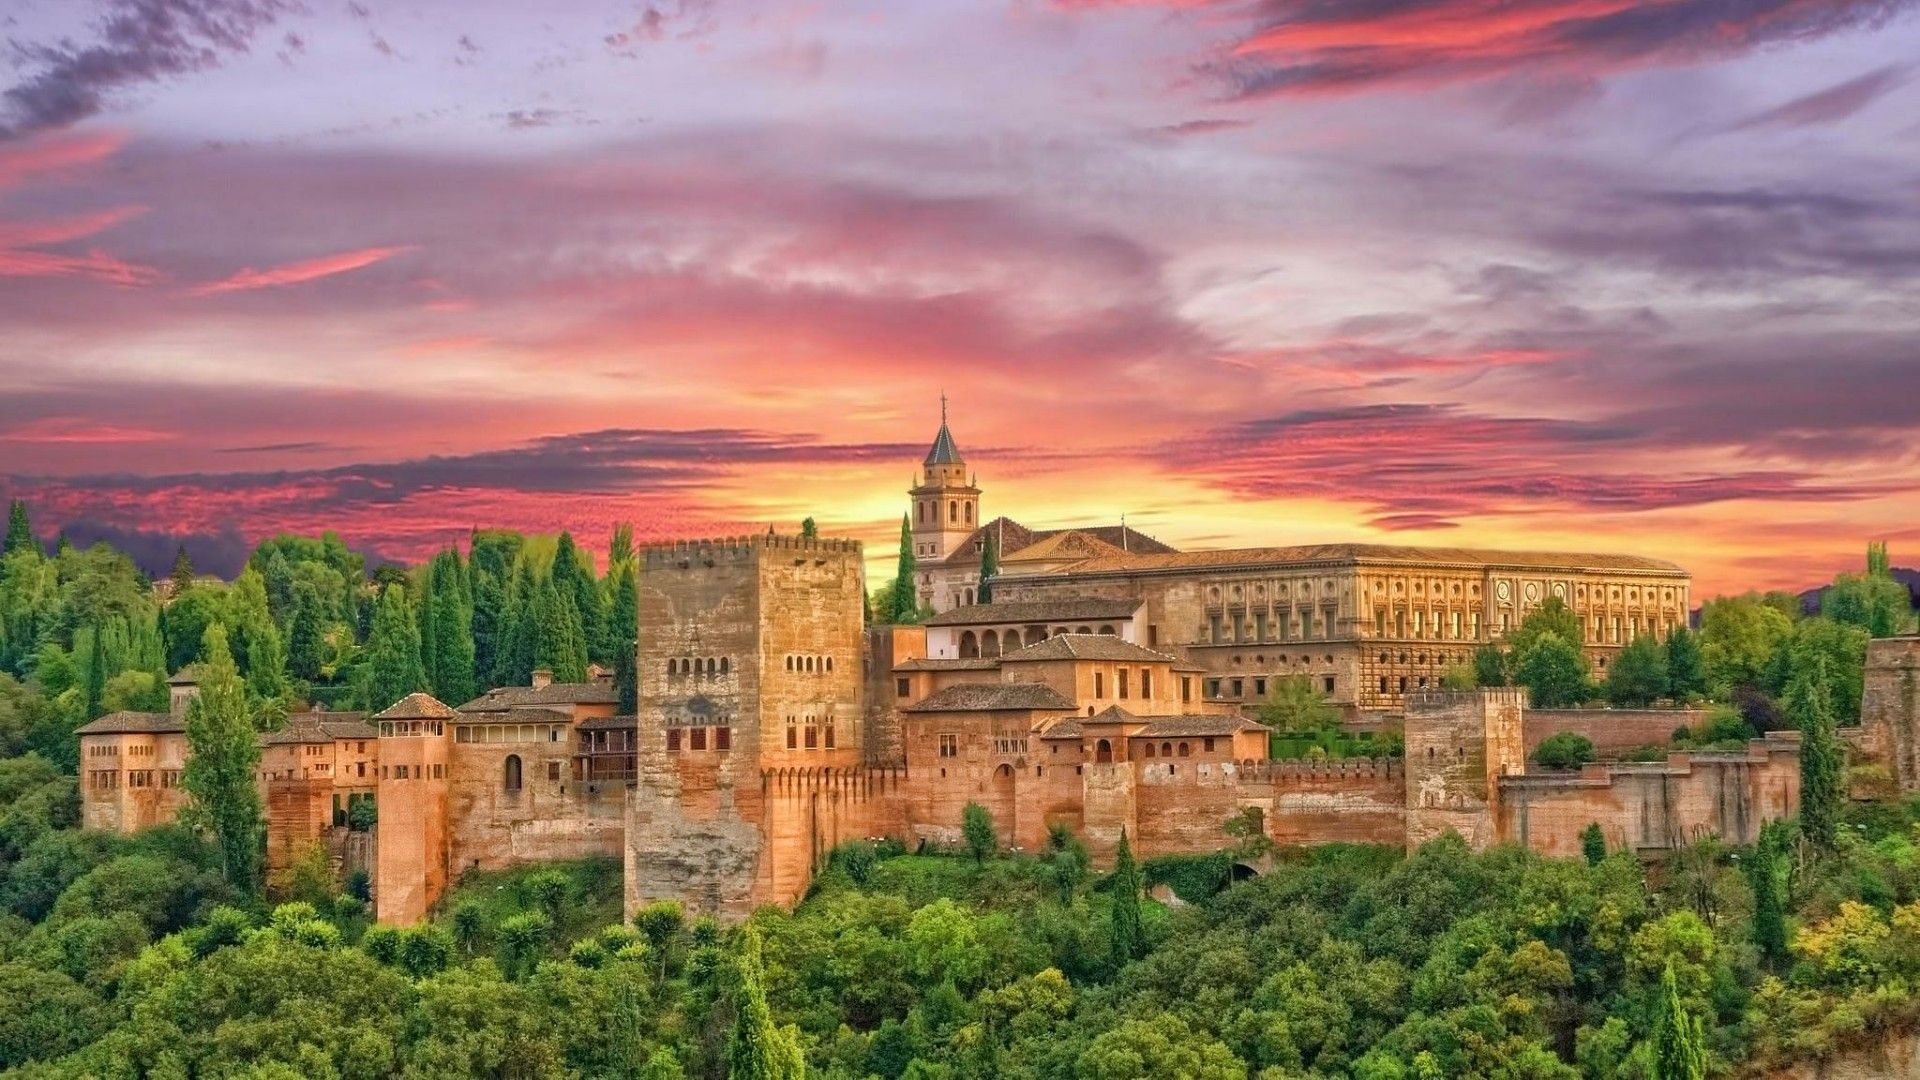
\includegraphics[width=\paperwidth,height=\paperheight,keepaspectratio]{images/granada.jpg}}
}

% Inicio del documento
\begin{document}

% Portada
\maketitle
\thispagestyle{empty}

\begin{center}
    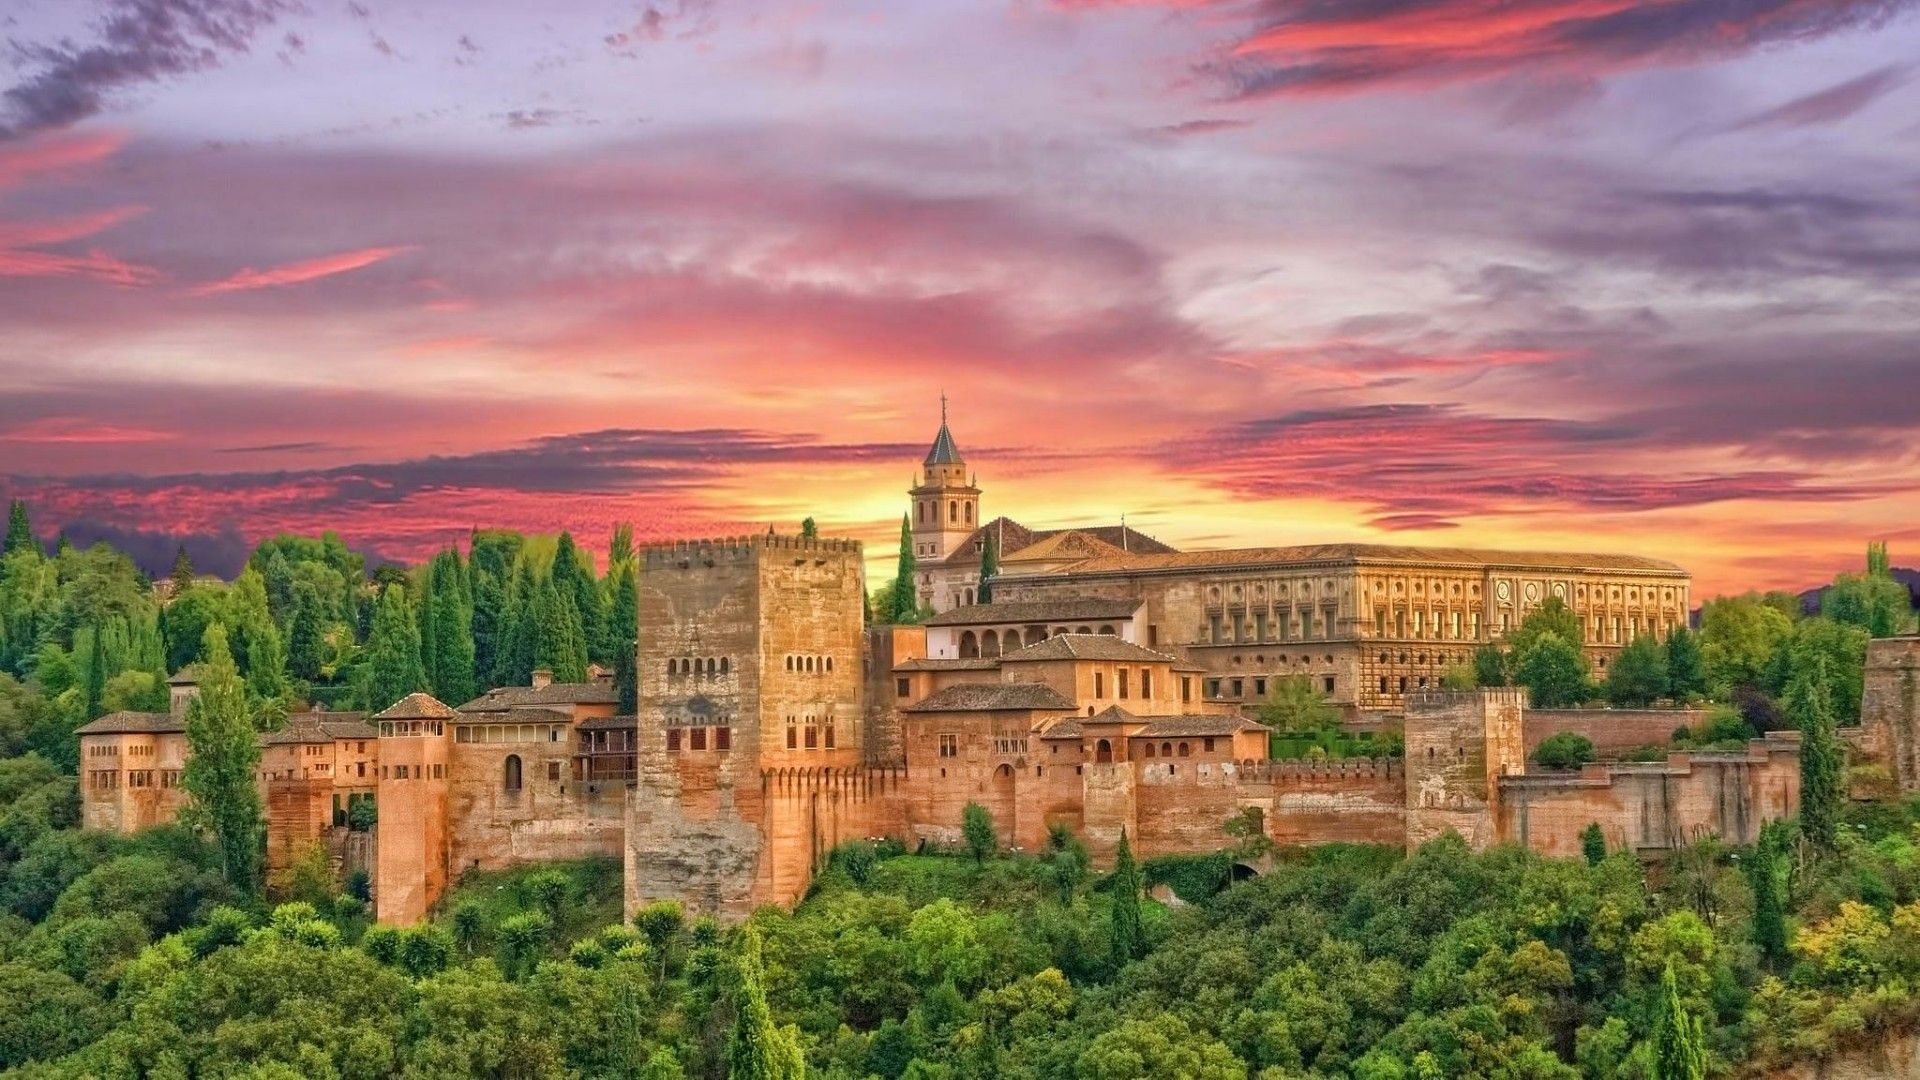
\includegraphics[width=\textwidth,height=0.4\textheight,keepaspectratio]{images/granada.jpg} \\ % Añade tu imagen de fondo
    \vfill
\end{center}

\newpage

% Índice (opcional)
\tableofcontents
\newpage


\section{Introducción}

Una red de comunicaciones se considera \textbf{segura} cuando se garantiza la protección de todos los aspectos clave de la seguridad. Sin embargo, es importante destacar que \textbf{no existen protocolos ni redes 100\% seguras}.

\subsection{¿Qué es la seguridad?}

La seguridad en redes engloba múltiples aspectos fundamentales:

\begin{itemize}
    \item \textbf{Confidencialidad/Privacidad:} El contenido de la información debe ser comprensible únicamente para las entidades autorizadas.
    \item \textbf{Autenticación:} Garantiza que las entidades involucradas son quienes afirman ser.
    \item \textbf{Control de accesos:} Los servicios deben estar accesibles solo a entidades autorizadas.
    \item \textbf{No repudio o irrenunciabilidad:} Impide que una entidad niegue haber realizado una acción determinada.
    \item \textbf{Integridad:} El sistema debe detectar cualquier alteración de la información, ya sea intencionada o accidental.
    \item \textbf{Disponibilidad:} Los servicios deben mantenerse operativos, independientemente de la demanda.
\end{itemize}

\subsection{¿En qué nivel o capa se debe situar la seguridad?}

La seguridad debe aplicarse en \textbf{todas las capas del sistema}. El grado de seguridad siempre estará limitado por el punto más débil de la red.

\subsection{Mecanismos de Seguridad}

Para garantizar los aspectos mencionados, se utilizan los siguientes mecanismos:

\begin{itemize}
    \item \textbf{Cifrado:} Puede ser simétrico o asimétrico.
    \item \textbf{Autenticación con clave secreta:} Utilizando mecanismos de reto-respuesta.
    \item \textbf{Intercambio de Diffie-Hellman:} Permite establecer claves secretas de forma segura.
    \item \textbf{Funciones Hash:} Como el código de autenticación de mensajes (\textit{Hash Message Authentication Code, HMAC}).
    \item \textbf{Firma Digital:} Para garantizar la autenticidad e integridad de los mensajes.
    \item \textbf{Certificados Digitales:} Utilizados para validar identidades.
\end{itemize}

\subsection{Ataques de Seguridad}

Un \textbf{ataque de seguridad} se define como cualquier acción, intencionada o no, que compromete alguno de los aspectos de la seguridad. Entre los ataques más comunes se encuentran:

\begin{itemize}
    \item \textbf{Sniffing:} También conocido como ''escuchas'' o \textit{husmeo}, vulnera la confidencialidad al interceptar información.
    \item \textbf{Spoofing (phishing):} Suplantación de identidad de entidades legítimas.
    \item \textbf{Man in the Middle:} Ataques de interceptación donde un tercero se posiciona entre las entidades comunicantes.
    \item \textbf{Denegación de Servicio Distribuida (DDoS):} Ejemplo de este ataque es el \textit{flooding} o inundación de solicitudes para colapsar un sistema.
    \item \textbf{Malware:} Incluye amenazas como troyanos, gusanos, \textit{spyware}, puertas traseras (\textit{backdoors}), \textit{rootkits}, ransomware y \textit{keyloggers}.
\end{itemize}



\section{Cifrado}

\textbf{Cifrado de datos:}

\begin{itemize}
    \item Es un procedimiento diseñado para garantizar la \textbf{confidencialidad} de la información.
    \item Consiste en transformar un \textbf{texto llano o claro} (\(P\)) en un \textbf{texto cifrado} (\(C\)).
    \item Este proceso se basa en la utilización de un algoritmo de \textbf{cifrado/descifrado}, comúnmente representado como \(E_K()\) para cifrado y \(D_{K'}()\) para descifrado.
    \item La complejidad del proceso radica en la utilización de una \textbf{clave de cifrado} (\(K\)) y una \textbf{clave de descifrado} (\(K'\)), las cuales deben permanecer desconocidas para garantizar la seguridad del sistema.
\end{itemize}

\begin{figure}[H]
    \centering
    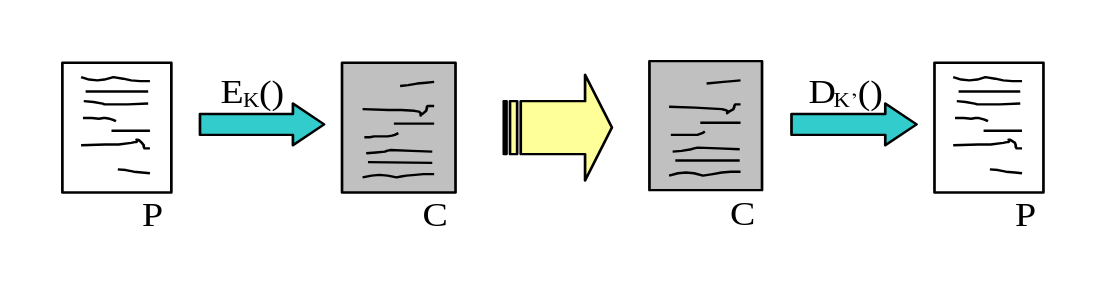
\includegraphics[width=0.8\textwidth]{images/cifrado.png}
    \caption{Esquema de cifrado de datos.}
\end{figure}
\newpage
\subsection{Cifrado simétrico}
\textbf{Cifrado simétrico: Algoritmos de clave secreta}

\begin{itemize}
    \item Utiliza una \textbf{única clave} para realizar tanto el cifrado como el descifrado, es decir, \(K = K'\).
    \item Un ejemplo representativo es el \textbf{DES} (\textit{Data Encryption Standard}), desarrollado por IBM en 1975.
\end{itemize}

\textbf{Enlaces relacionados:}
\begin{itemize}
    \item \href{http://en.wikipedia.org/wiki/Feistel_network}{Estructura Feistel}\footnote{Puedes pinchar en los nombres para acceder a los enlaces}: Explicación de la arquitectura utilizada en muchos algoritmos de cifrado, incluido DES.
    \item \href{http://en.wikipedia.org/wiki/Data_Encryption_Standard}{Data Encryption Standard}: Detalles técnicos y evolución histórica del algoritmo.
\end{itemize}


\begin{figure}[H]
    \centering
    \begin{minipage}{0.45\textwidth}
        \centering
        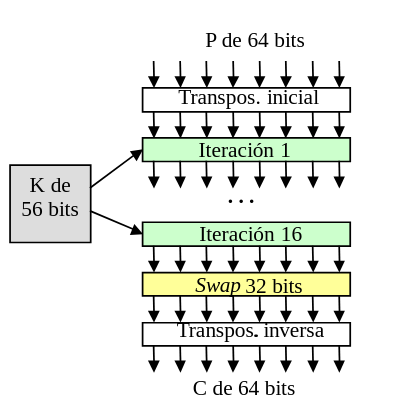
\includegraphics[width=\textwidth]{images/crifrado_a.png}
        \caption{Diagrama A}
    \end{minipage}
    \hfill
    \begin{minipage}{0.45\textwidth}
        \centering
        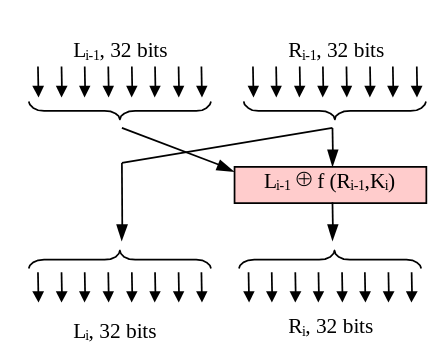
\includegraphics[width=\textwidth]{images/cifrado_b.png}
        \caption{Diagrama B}
    \end{minipage}
\end{figure}

\begin{itemize}
    \item Diagrama A:
    \begin{itemize}
        \item \textbf{P de 64 bits} (plaintext) pasa por una \textbf{Transpos. inicial} (permutación inicial).
        \item El resultado se somete a 16 iteraciones (\textbf{Iteración 1} a \textbf{Iteración 16}) utilizando una \textbf{K de 56 bits} (clave de 56 bits).
        \item Después de las iteraciones, ocurre un \textbf{Swap 32 bits}.
        \item Finalmente, se aplica la \textbf{Transpos. inversa} (permutación inversa) para producir el \textbf{C de 64 bits} (ciphertext).
    \end{itemize}
    \item Diagrama B:
    \begin{itemize}
        \item El \textbf{entrada de 64 bits} se divide en dos mitades de 32 bits, \textbf{Li-1, 32 bits} y \textbf{Ri-1, 32 bits}.
        \item \textbf{Li-1} se combina con el resultado de una función \textbf{f} aplicada a \textbf{Ri-1} y una subclave \textbf{Ki} usando la operación XOR (\(\oplus\)).
        \item La salida es dos mitades de 32 bits, \textbf{Li, 32 bits} y \textbf{Ri, 32 bits}.
    \end{itemize}        
\end{itemize}

\begin{itemize}
    \item \textbf{DES:} Es un esquema de \textbf{sustitución monoalfabética}, lo que significa que cada símbolo del texto plano se sustituye por otro, según un esquema fijo basado en la clave.
    \item \textbf{Encadenamiento DES:} Introducido para evitar que DES actúe como un simple algoritmo de sustitución. Este mecanismo encadena los bloques cifrados, asegurando que cada bloque de texto cifrado dependa no solo del bloque actual de texto claro, sino también del bloque anterior de texto cifrado. Esto incrementa significativamente la seguridad del algoritmo.
    \item Para mejorar la robustez del cifrado, se utilizan variantes como \textbf{2DES} y \textbf{3DES}. 
    \begin{itemize}
        \item \textbf{2DES (Double DES):} Consiste en aplicar el algoritmo DES dos veces consecutivas con dos claves diferentes. Aunque incrementa la seguridad en comparación con DES simple, sigue siendo vulnerable a ciertos tipos de ataques, como el ataque de encuentro en el medio (\textit{meet-in-the-middle}).
        \item \textbf{3DES (Triple DES):} Aplica el algoritmo DES tres veces, generalmente con dos o tres claves diferentes. Este método es mucho más seguro que DES y 2DES, y ha sido ampliamente utilizado en la industria para proteger datos sensibles.
    \end{itemize}
\end{itemize}

\begin{figure}[H]
    \centering
    \begin{minipage}{0.45\textwidth}
        \centering
        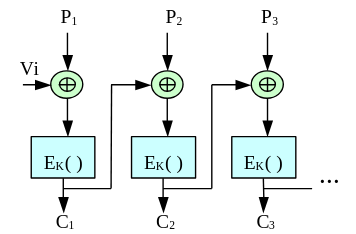
\includegraphics[width=\textwidth]{images/des_A.png}
        \caption{Diagrama A}
    \end{minipage}
    \hfill
    \begin{minipage}{0.45\textwidth}
        \centering
        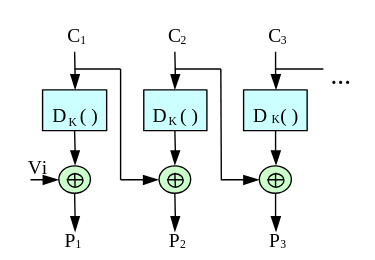
\includegraphics[width=\textwidth]{images/des_B.png}
        \caption{Diagrama B}
    \end{minipage}
    \hfill
    \begin{minipage}{0.6\textwidth}
        \centering
        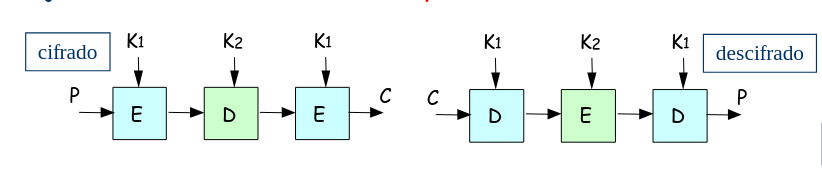
\includegraphics[width=\textwidth]{images/des2_y_3des.png}
        \caption{Diagrama 2 y 3DES}
    \end{minipage}
\end{figure}


\newpage

\textbf{IDEA (\textit{International Data Encryption Algorithm, IDEA})}

\begin{itemize}
    \item Es un algoritmo de cifrado \textbf{simétrico}, lo que significa que utiliza la \textbf{misma clave} tanto para cifrar como para descifrar.
    \item Utiliza \textbf{claves de 128 bits}, proporcionando un alto nivel de seguridad.
    \item Diseñado para \textbf{operar en tiempo real}, con implementación eficiente en hardware (\textit{Very Large Scale Integration, VLSI}).
\end{itemize}

\begin{figure}[H]
    \centering
    \begin{minipage}{0.45\textwidth}
        \centering
        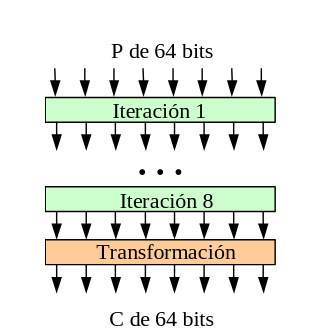
\includegraphics[width=\textwidth]{images/ideaA.png}
        \caption{Diagrama A}
    \end{minipage}
    \hfill
    \begin{minipage}{0.45\textwidth}
        \centering
        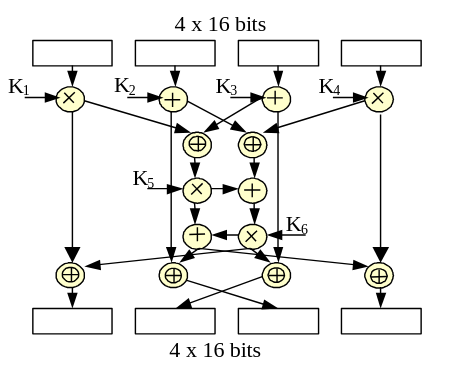
\includegraphics[width=\textwidth]{images/ideaB.png}
        \caption{Diagrama B}
    \end{minipage}
\end{figure}

\subsection{Cifrado asimétrico}

\textbf{Cifrado asimétrico: Algoritmos de clave pública/privada}

\begin{itemize}
    \item Cada usuario (\(A\)) posee dos claves distintas:
    \begin{itemize}
        \item Una \textbf{clave pública} (\(K_{\text{PUB}_A}\)).
        \item Una \textbf{clave privada} (\(K_{\text{PRI}_A}\)).
    \end{itemize}
    \item Conociendo \(K_{\text{PUB}_A}\), es \textbf{imposible deducir} \(K_{\text{PRI}_A}\).
    \item Las claves son diferentes para las operaciones de cifrado y descifrado:
    \begin{itemize}
        \item \textbf{Cifrado:} \(C = E_{K_{\text{PUB}_B}}(P)\), donde \(P\) es el texto plano.
        \item \textbf{Descifrado:} \(P = D_{K_{\text{PRI}_B}}(C)\), donde \(C\) es el texto cifrado.
    \end{itemize}
    \item En caso de enviar \(C = E_{K_{\text{PRI}_A}}(P)\), el receptor puede verificar la \textbf{autenticidad} del mensaje al descifrarlo con \(K_{\text{PUB}_A}\).
\end{itemize}

\begin{figure}[H]
    \centering
    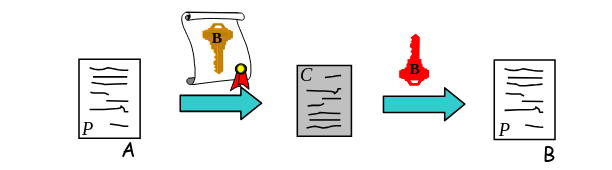
\includegraphics[width=0.8\textwidth]{images/cifrado_asimetrico.png}
    \caption{Esquema de cifrado asimétrico.}
\end{figure}

\textbf{RSA (\textit{Rivest, Shamir y Adleman})}

\begin{itemize}
    \item Se eligen dos números primos grandes \(p\) y \(q\), donde \(p, q > 10^{100}\).
    \item Calculamos:
    \begin{itemize}
        \item \(n = p \cdot q\).
        \item \(z = (p-1) \cdot (q-1)\), utilizando la función de Euler.
    \end{itemize}
    \item Elegimos un número \(d\), primo respecto de \(z\).
    \item Calculamos \(e\) tal que \(e \cdot d \mod z = 1\), utilizando el algoritmo de Euclides.
    \item Las claves generadas son:
    \begin{itemize}
        \item Clave pública: \(K_{\text{PUB}} = (e, n)\).
        \item Clave privada: \(K_{\text{PRI}} = (d, n)\).
    \end{itemize}
    \item Las operaciones de cifrado y descifrado son:
    \begin{itemize}
        \item \textbf{Cifrado:} \(C = P^e \mod n\).
        \item \textbf{Descifrado:} \(P = C^d \mod n\).
    \end{itemize}
\end{itemize}

\textbf{Ejemplo RSA}

\begin{itemize}
    \item Se eligen los valores:
    \begin{itemize}
        \item \(p = 3\), \(q = 11\).
        \item \(n = p \cdot q = 33\).
        \item \(z = (p-1)(q-1) = (3-1)(11-1) = 2 \cdot 10 = 20\).
    \end{itemize}
    \item Elegimos \(d = 7\), un número primo respecto de \(z\).
    \item Calculamos \(e\) tal que \(e \cdot d \mod z = 1\). En este caso, \(e = 3\).
    \item Las claves generadas son:
    \begin{itemize}
        \item Clave pública: \(K_{\text{PUB}} = (3, 33)\).
        \item Clave privada: \(K_{\text{PRI}} = (7, 33)\).
    \end{itemize}
\end{itemize}

\textbf{Cifrado y descifrado}

La siguiente tabla muestra el proceso de cifrado y descifrado para varios caracteres. Utilizamos la notación:

\begin{itemize}
    \item \textbf{Cifrado:} \(C = P^e \mod n\).
    \item \textbf{Descifrado:} \(P = C^d \mod n\).
\end{itemize}

\begin{figure}[H]
    \centering
    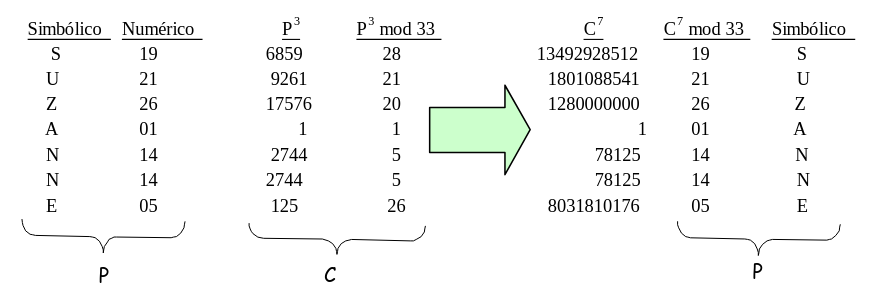
\includegraphics[width=0.8\textwidth]{images/rsa.png}
    \caption{Ejercicio Resuelto RSA.}
\end{figure}

\textbf{Resultado:} El texto original se recupera perfectamente después del cifrado y descifrado, demostrando la efectividad del esquema RSA.

\section{Autenticación}
\subsection{Reto-respuesta}

\begin{itemize}
    \item \textbf{Esquema de reto-respuesta:}
    \begin{itemize}
        \item Este método se utiliza para verificar la identidad de una entidad (por ejemplo, un cliente o servidor) sin necesidad de compartir directamente la clave secreta.
        \item El procedimiento típico es:
        \begin{enumerate}
            \item La entidad que autentica (por ejemplo, el servidor) envía un \textbf{reto} (\(R\)) a la otra entidad (por ejemplo, el cliente).
            \item El cliente responde cifrando el reto con la clave secreta compartida (\(K\)), generando la respuesta cifrada \(C = E_K(R)\).
            \item El servidor descifra la respuesta con la clave compartida y verifica si coincide con el reto original.
        \end{enumerate}
    \end{itemize}
    \item \textbf{¿Ataque por reflexión?}
    \begin{itemize}
        \item Un ataque por reflexión ocurre cuando un atacante intercepta un reto enviado por una entidad y lo devuelve como respuesta, intentando hacerse pasar por una entidad legítima.
        \item Para mitigar este ataque, es importante implementar:
        \begin{itemize}
            \item \textbf{Espacios de claves disjuntos:} Utilizar claves diferentes para cada dirección de comunicación. Por ejemplo:
            \begin{itemize}
                \item \(K_{A \to B}\): Clave utilizada para mensajes enviados de \(A\) a \(B\).
                \item \(K_{B \to A}\): Clave utilizada para mensajes enviados de \(B\) a \(A\).
            \end{itemize}
            \item Esto garantiza que un reto enviado por \(A\) no pueda ser simplemente reflejado de vuelta a \(A\) por \(B\), ya que \(A\) esperará que el mensaje esté cifrado con \(K_{B \to A}\).
        \end{itemize}
    \end{itemize}
\end{itemize}

\textbf{Resumen:} El esquema de reto-respuesta ofrece una manera eficiente de autenticar entidades sin revelar claves secretas. Sin embargo, es crucial implementar contramedidas como los \textbf{espacios de claves disjuntos} para evitar ataques por reflexión.

\begin{figure}[H]
    \centering
    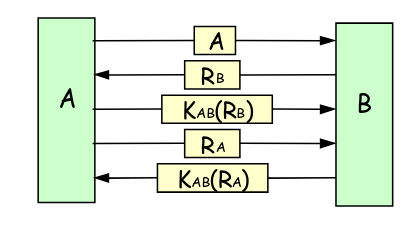
\includegraphics[width=0.8\textwidth]{images/reto_respuesta.png}
    \caption{Esquema de reto-respuesta.}
\end{figure}

\subsection{Intercambio de Diffie-Hellman}

El \textit{intercambio de claves de Diffie-Hellman} es un protocolo de criptografía que permite a dos entidades, A y B, establecer una clave secreta compartida, sin necesidad de intercambiar dicha clave explícitamente. En su lugar, utilizan números públicos y realizan cálculos sobre ellos. A continuación se describen los pasos básicos del protocolo:

\begin{enumerate}
    \item Ambas partes acuerdan un número primo grande \( p \) y una base \( g \), los cuales son públicos.
    \item La parte A elige un número secreto \( a \) y calcula \( A = g^a \mod p \), luego envía \( A \) a la parte B.
    \item La parte B elige un número secreto \( b \) y calcula \( B = g^b \mod p \), luego envía \( B \) a la parte A.
    \item Ambas partes calculan la clave compartida:
    \begin{itemize}
        \item La parte A calcula \( K = B^a \mod p \).
        \item La parte B calcula \( K = A^b \mod p \).
    \end{itemize}
    Como \( A^b \mod p = B^a \mod p \), ambas partes obtienen la misma clave secreta \( K \), que pueden usar para cifrar la comunicación.
\end{enumerate}

Este protocolo es seguro debido a la dificultad del problema de calcular los logaritmos discretos, es decir, dado \( g^a \mod p \) y \( g^b \mod p \), es extremadamente difícil calcular \( a \) o \( b \).

\begin{figure}[H]
    \centering
    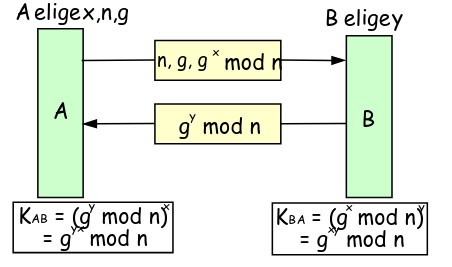
\includegraphics[width=0.8\textwidth]{images/diffie_hellman.png}
    \caption{Intercambio de claves de Diffie-Hellman.}
\end{figure}


\subsubsection{Ataque Man-in-the-Middle (MitM)}

Aunque el intercambio de Diffie-Hellman es seguro, puede ser vulnerable a un \textit{ataque Man-in-the-Middle} (MitM). En este tipo de ataque, un atacante (C) se coloca entre las dos partes A y B, interceptando y alterando los mensajes entre ellas.

\begin{enumerate}
    \item La parte A envía su valor \( A = g^a \mod p \) al atacante (C) en lugar de enviarlo directamente a B.
    \item El atacante (C) elige su propio valor secreto \( c \), calcula \( C = g^c \mod p \) y envía \( C \) a la parte B.
    \item La parte B, al recibir \( C \), calcula la clave \( K_B = C^b \mod p \) y la envía de vuelta al atacante.
    \item El atacante calcula la clave \( K_A = A^c \mod p \), y ahora tiene dos claves secretas: \( K_A \) y \( K_B \).
    \item De esta manera, el atacante puede leer y modificar la comunicación entre A y B sin que ninguna de las partes se dé cuenta.
\end{enumerate}

Este ataque funciona porque A y B creen que están intercambiando información directamente entre sí, pero en realidad están enviando la información al atacante, quien actúa como intermediario.

Para mitigar este tipo de ataque, se pueden usar firmas digitales o certificados, lo que permite a A y B asegurarse de que están comunicándose con la parte correcta.

\begin{figure}[H]
    \centering
    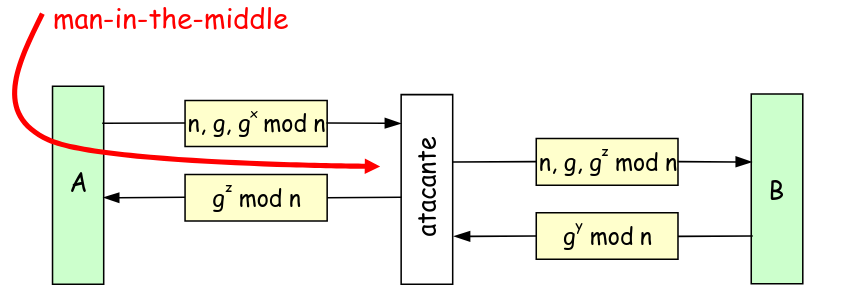
\includegraphics[width=0.8\textwidth]{images/ataque.png}
    \caption{Ataque}
\end{figure}

\section{Funciones Hash}

\subsection{Funciones Hash (Compendios)}

Las funciones hash son algoritmos matemáticos que transforman un mensaje de longitud variable en una secuencia de longitud fija. Son ampliamente utilizadas en criptografía para garantizar la integridad de los datos y otros aspectos de seguridad.

\subsubsection{Características de los Compendios}

Las funciones hash tienen las siguientes características:

\begin{itemize}
    \item \textbf{Funciones unidireccionales (irreversibles):} El cálculo de un hash es sencillo, pero es prácticamente imposible obtener el mensaje original a partir de su resumen hash.
    \item \textbf{Texto de entrada (M) de longitud variable:} El tamaño del mensaje de entrada puede variar, pero siempre se transforma en un resumen de longitud fija.
    \item \( M \rightarrow H(M) \): El mensaje \( M \) se convierte en un hash \( H(M) \), que tiene una longitud fija (por ejemplo, 256 o 512 bits).
    \item \textbf{Imposibilidad de obtener \( M \) a partir de \( H(M) \):} Dado un hash \( H(M) \), es prácticamente imposible encontrar el mensaje \( M \) original.
    \item \textbf{Invulnerabilidad a ataques de colisión:} Es imposible encontrar dos mensajes diferentes, \( M \) y \( M' \), que produzcan el mismo hash \( H(M) = H(M') \).
\end{itemize}

\subsubsection{Ejemplos de Funciones Hash}

Algunos ejemplos de funciones hash populares son:

\begin{itemize}
    \item MD5
    \item SHA-1
    \item SHA-512
\end{itemize}

\subsubsection{Uso de las Funciones Hash}

Las funciones hash se utilizan principalmente para garantizar la integridad de los datos y la autenticación. Un ejemplo común es el \textit{Hash Message Authentication Code} (HMAC), que combina un mensaje \( M \) con una clave \( K \):

\[
HMAC(K, M) = H(K \parallel M)
\]

Para evitar ataques de extensión, se utiliza una versión más segura:

\[
HMAC(K, M) = H(K \parallel H(K \parallel M))
\]

\subsubsection{MD5 (Message Digest 5, RFC 1321)}

El proceso de generación de un resumen MD5\footnote{Para imágenes de ellos accede a la diapostiva 21 del tema 4} de 128 bits se realiza en los siguientes pasos:

\begin{itemize}
    \item \textbf{Relleno:} El mensaje se rellena con 100..0 hasta alcanzar una longitud máxima de 448 bits.
    \item \textbf{Adición de campo de longitud:} Se añade un campo de 64 bits que contiene la longitud original del mensaje.
    \item \textbf{División en bloques:} El mensaje se divide en bloques de 512 bits.
    \item \textbf{Procesamiento secuencial:} Los bloques se procesan secuencialmente para generar el resumen de 128 bits.
\end{itemize}

\subsubsection{SHA-1 (Secure Hash Algorithm 1, NIST 1993)}

El proceso de generación de un resumen SHA-1\footnote{Para imágenes de ellos accede a la diapostiva 22 del tema 4} de 160 bits es muy similar al de MD5:

\begin{itemize}
    \item \textbf{Relleno:} El mensaje se rellena con 100..0 hasta alcanzar una longitud máxima de 448 bits.
    \item \textbf{Adición de campo de longitud:} Se añade un campo de 64 bits que contiene la longitud original del mensaje.
    \item \textbf{División en bloques:} El mensaje se divide en bloques de 512 bits.
    \item \textbf{Procesamiento secuencial:} Los bloques se procesan secuencialmente para generar el resumen de 160 bits.
\end{itemize}

\section{Firma Digital y certificados digitales}

\subsection{Firma Digital: Objetivos}

La firma digital tiene varios objetivos clave en el contexto de la seguridad y la autenticación:

\begin{itemize}
    \item \textbf{El receptor pueda autenticar al emisor:} La firma digital permite que el receptor verifique la identidad del emisor.
    \item \textbf{No haya repudio:} El emisor no puede negar la autenticidad del mensaje firmado, ya que solo él podría haber firmado ese mensaje con su clave privada.
    \item \textbf{El emisor tenga garantías de no falsificación (integridad):} La firma garantiza que el mensaje no ha sido alterado desde que fue firmado.
\end{itemize}

\subsubsection{Firma Digital con Clave Secreta y Asimétrica}

Existen dos tipos de firmas digitales, dependiendo del sistema de claves utilizado:

\begin{itemize}
    \item \textbf{Firma digital con clave secreta:} Usada en sistemas donde se utiliza una sola clave para cifrar y descifrar.
    Cabe destacar el ejemplo de Big Brother, que realiza diversas operaciones hashing para la clave secreta de la firma digital.
    \begin{figure}[H]
        \centering
        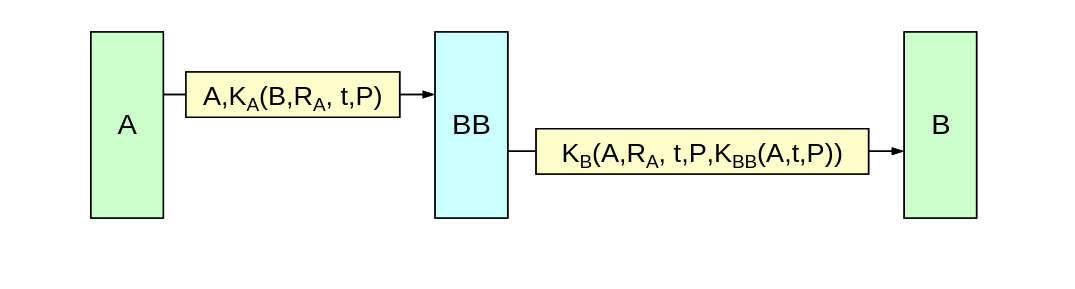
\includegraphics[width=0.8\textwidth]{images/big_brother.png}
        \caption{Big Brother}
    \end{figure}
    \item \textbf{Firma digital con clave asimétrica:} Se utilizan dos claves, una pública y otra privada. El emisor firma el mensaje con su clave privada y el receptor verifica la firma con la clave pública del emisor.
\end{itemize}

\subsubsection{El concepto de \textit{Big Brother} en la firma digital}

El concepto de \textit{Big Brother} en la firma digital se refiere a un escenario donde una autoridad central o entidad de confianza supervisa, regula y controla el proceso de autenticación y verificación de firmas digitales. Esta idea se asemeja a un sistema donde todos los actores confían en una única entidad para garantizar la seguridad e integridad de las operaciones. A continuación, se describen los pasos fundamentales en este esquema:

\begin{enumerate}
    \item \textbf{Generación de claves:} Cada usuario genera un par de claves criptográficas (una clave pública y una clave privada). La clave pública es registrada y almacenada por la autoridad central (el \textit{Big Brother}).
    \item \textbf{Emisión de certificados:} La autoridad central emite certificados digitales para asociar cada clave pública con la identidad del usuario. Estos certificados son firmados digitalmente por la autoridad, lo que les otorga validez y confiabilidad.
    \item \textbf{Creación de la firma:} Para firmar un documento, el usuario utiliza su clave privada. Este proceso produce una firma digital única, basada en el contenido del documento y en la clave privada del usuario.
    \item \textbf{Verificación de la firma:} La parte receptora utiliza la clave pública del usuario para verificar la autenticidad de la firma digital. La validez de la clave pública y su asociación con la identidad del firmante se confirman consultando el certificado digital emitido por la autoridad central.
    \item \textbf{Control y supervisión:} La autoridad central actúa como un garante del sistema, asegurando que las claves públicas y los certificados estén actualizados y evitando posibles fraudes o duplicaciones.
\end{enumerate}

Este modelo tiene la ventaja de centralizar la confianza, simplificando el proceso para los usuarios finales. Sin embargo, también presenta desafíos significativos, como la dependencia total de la autoridad central, que puede convertirse en un único punto de falla en el sistema.
\newpage




El proceso de firma digital con clave asimétrica se puede describir mediante un doble cifrado:

\begin{figure}[H]
    \centering
    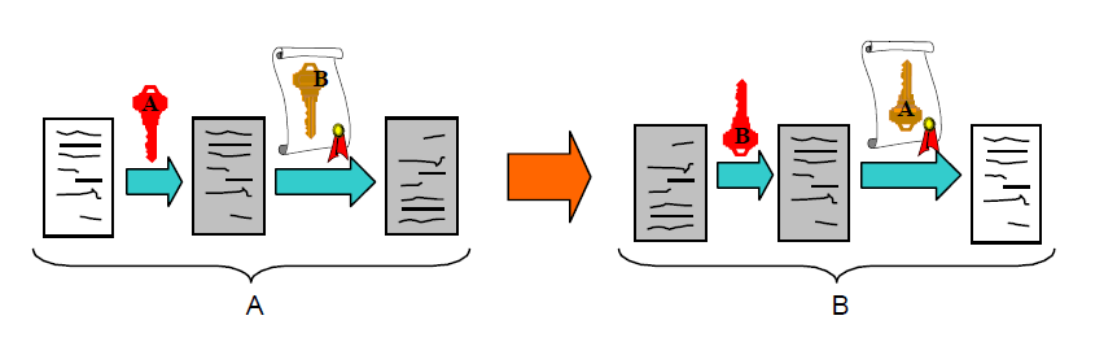
\includegraphics[width=0.8\textwidth]{images/cifrado_ej.png}
    \caption{Proceso de firma digital con clave asimétrica.}
\end{figure}

\begin{enumerate}
    \item Primero, para proporcionar privacidad, el mensaje \( T \) es cifrado con la clave pública \( K_{\text{pubB}} \) del receptor.
    \item Luego, para autenticación, se cifra previamente con la clave privada \( K_{\text{priA}} \) del emisor.
    \item El mensaje firmado se envía como \( K_{\text{pubB}}( K_{\text{priA}}( T ) ) \).
    \item El receptor, al recibir el mensaje, lo descifra primero con su clave privada \( K_{\text{priB}} \), luego con la clave pública del emisor \( K_{\text{pubA}} \), y finalmente obtiene el mensaje original \( T \).
\end{enumerate}



\subsubsection{Debilidad y Garantía de No Repudio}

Una de las debilidades del sistema es que para garantizar el \textit{no repudio}, se necesita asegurar la asociación indisoluble entre la ''identidad A'' y su ''clave pública \( K_{\text{pubA}} \)''. Esto es necesario para garantizar que el emisor no pueda negar su identidad al haber firmado el mensaje.

Para resolver este problema, se utiliza un \textit{certificado digital}, que garantiza la asociación entre una identidad y una clave pública.

\subsubsection{Certificados Digitales}

Un \textit{certificado digital} es un documento que asocia de manera fidedigna una identidad a una clave pública. El proceso de obtención y verificación de un certificado digital incluye los siguientes pasos:

\begin{itemize}
    \item El usuario genera su par de claves pública y privada.
    \item El usuario envía una solicitud a una \textit{Autoridad de Certificación} (AC), firmada digitalmente, indicando su identidad y su clave pública.
    \item La AC verifica la firma y, si todo es correcto, emite un certificado digital que contiene:
    \begin{itemize}
        \item La identidad de la AC.
        \item La identidad del usuario.
        \item La clave pública del usuario.
        \item Otros datos, como el período de validez del certificado.
    \end{itemize}
    \item El certificado es firmado digitalmente por la AC, utilizando su clave privada, para evitar su falsificación.
\end{itemize}

\subsubsection{Formato de los Certificados}

El formato más común para los certificados digitales es el estándar \textit{X.509}. Este formato asegura que los certificados sean compatibles entre diferentes sistemas y aplicaciones.

\subsubsection{Autoridades de Certificación (AC) Reconocidas}

Algunas de las Autoridades de Certificación más reconocidas incluyen:

\begin{itemize}
    \item ACE (www.ace.es)
    \item VeriSign (www.verisign.com)
    \item CAMERFIRMA (www.camerfirma.es)
    \item CERES (www.cert.fnmt.es)
\end{itemize}

\subsubsection{Campos de un certificado \textit{X.509}}

\begin{figure}[H]
    \centering
    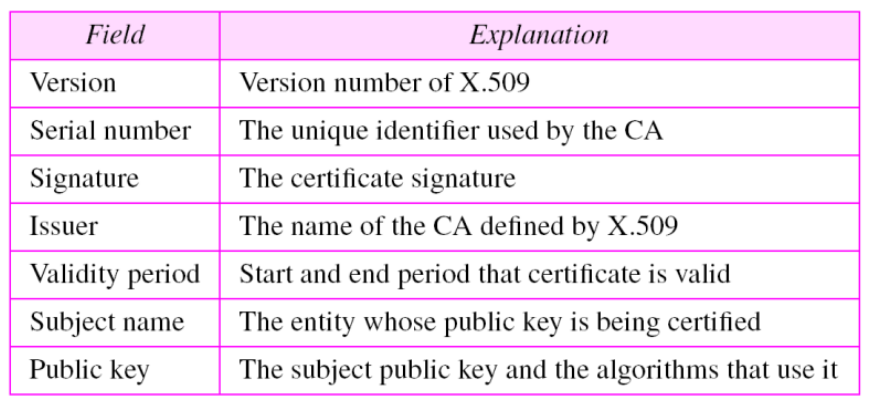
\includegraphics[width=0.8\textwidth]{images/campos_certificado.png}
    \caption{Campos de un certificado X.509.}
\end{figure}

\footnotetext{Para más información de un certificado X.509 accede a la diapositiva 28 del tema 4.}

\subsection{Relación entre los Mecanismos de Seguridad y los Servicios/Aspectos de Seguridad}

Existen varios mecanismos de seguridad que ayudan a garantizar los diferentes aspectos de la seguridad en los sistemas informáticos. A continuación, se describe la relación entre los mecanismos de seguridad y los servicios de seguridad más importantes:

\subsubsection{Confidencialidad}

La \textit{confidencialidad} se refiere a garantizar que solo las partes autorizadas puedan acceder a la información. Se consigue mediante el uso de cifrado, que puede ser de dos tipos:

\begin{itemize}
    \item \textbf{Cifrado simétrico:} Utiliza una única clave secreta compartida entre el emisor y el receptor para cifrar y descifrar el mensaje.
    \item \textbf{Cifrado asimétrico:} Utiliza un par de claves, una pública y una privada, donde el emisor cifra el mensaje con la clave pública del receptor y el receptor descifra con su clave privada.
\end{itemize}

Ambos métodos permiten garantizar que la información permanezca confidencial durante su transmisión.

\subsubsection{Autenticación}

La \textit{autenticación} asegura que el receptor pueda verificar la identidad del emisor. Se consigue mediante varios mecanismos, como:

\begin{itemize}
    \item \textbf{Reto-respuesta:} El receptor envía un reto (por ejemplo, una pregunta o desafío) al emisor, quien debe responder correctamente para probar su identidad.
    \item \textbf{Firma digital (Big Brother, doble cifrado):} La firma digital asegura que un mensaje provenga de una fuente específica. En el doble cifrado, el mensaje es cifrado primero con la clave pública del receptor para garantizar la privacidad y luego con la clave privada del emisor para garantizar la autenticidad.
\end{itemize}

\subsubsection{No Repudio}

El \textit{no repudio} significa que el emisor no puede negar haber enviado un mensaje una vez que ha sido firmado. Este aspecto de la seguridad se logra mediante:

\begin{itemize}
    \item \textbf{Firma digital (Big Brother, doble cifrado):} Al firmar digitalmente un mensaje con la clave privada del emisor, se asegura que solo él pudo haberlo firmado, lo que impide que pueda negar su participación en la transmisión del mensaje.
\end{itemize}

\subsubsection{Integridad}

La \textit{integridad} garantiza que el mensaje no haya sido alterado durante la transmisión. Se consigue mediante:

\begin{itemize}
    \item \textbf{Compendios o resúmenes:} Se genera un valor hash del mensaje utilizando funciones hash. Este valor se adjunta al mensaje como un resumen, y cualquier alteración del mensaje cambiará el resumen, lo que permite detectar la manipulación.
\end{itemize}

\subsubsection{Disponibilidad}

La \textit{disponibilidad} se refiere a asegurar que los servicios y recursos estén disponibles para los usuarios autorizados cuando los necesiten. Sin embargo, los mecanismos de seguridad mencionados anteriormente no proporcionan disponibilidad por sí solos. Para garantizar la disponibilidad, se requieren:

\begin{itemize}
    \item \textbf{Sistemas antiataque:} Para proteger contra ataques de denegación de servicio (DoS) y otros que puedan afectar la disponibilidad.
    \item \textbf{Redundancia:} La redundancia en las líneas de acceso y en los servidores garantiza que, en caso de fallo de un sistema, otro pueda tomar su lugar y continuar brindando los servicios.
\end{itemize}

\section{Protocolos Seguros}

\subsection{Seguridad}

\subsection*{Seguridad Perimetral}

La \textit{seguridad perimetral} se refiere a la protección de las redes de comunicaciones de una organización contra accesos no autorizados o ataques desde el exterior. Para ello, se utilizan diversos mecanismos de seguridad, entre los que destacan:

\begin{itemize}
    \item \textbf{Firewalls:} Son dispositivos o software que filtran el tráfico de red entre diferentes zonas, como la red interna y la externa, permitiendo o bloqueando conexiones según un conjunto de reglas predefinidas.
    \item \textbf{Sistemas de detección de intrusiones (IDS):} Son sistemas que monitorean el tráfico de red en busca de patrones o comportamientos sospechosos que puedan indicar un intento de intrusión.
    \item \textbf{Sistemas de respuesta a intrusiones (IRS):} Estos sistemas no solo detectan intrusiones, sino que también responden a ellas de manera automática, por ejemplo, bloqueando el acceso a ciertos recursos o alertando a los administradores.
\end{itemize}

\subsection*{Seguridad Criptográfica en Protocolos}

La seguridad en los protocolos de comunicación se puede aplicar en diferentes capas del modelo OSI, cada una con sus propias soluciones de seguridad:

\subsubsection*{Capa de Aplicación}

En la capa de aplicación se implementan mecanismos de seguridad para proteger las comunicaciones a nivel de la aplicación. Algunos ejemplos son:

\begin{itemize}
    \item \textbf{Pretty Good Privacy (PGP):} Es un protocolo de cifrado utilizado para la protección de correos electrónicos. PGP ofrece confidencialidad mediante cifrado, autenticación mediante firma digital y garantiza la integridad del mensaje mediante un hash.
    \item \textbf{Secure Shell (SSH):} Protocolo utilizado para acceder de manera segura a máquinas remotas, proporcionando cifrado de los datos, autenticación del servidor y del cliente, y confidencialidad en la comunicación.
\end{itemize}

\subsubsection*{Capa de Sesión (Entre Aplicación y Transporte)}

En esta capa, la seguridad se implementa mediante protocolos que proporcionan seguridad en la comunicación entre la capa de aplicación y la capa de transporte:

\begin{itemize}
    \item \textbf{Transport Layer Security (TLS):} Es un protocolo criptográfico que proporciona seguridad en las comunicaciones a través de la red. TLS, que anteriormente era conocido como SSL (Secure Sockets Layer), se utiliza en protocolos como HTTPS, IMAPS, SSL-POP y VPN. TLS ofrece:
    \begin{itemize}
        \item \textbf{Confidencialidad:} Mediante una clave secreta negociada entre el cliente y el servidor.
        \item \textbf{Autenticación:} El servidor se autentica por defecto mediante su clave pública (KPUBLICA).
        \item \textbf{Integridad:} Utilizando el algoritmo HMAC (Hash-based Message Authentication Code) para asegurar que los datos no han sido modificados durante la transmisión.
    \end{itemize}
    \item \textbf{TLS Handshake:} El proceso de \textit{Handshake} se utiliza para negociar los parámetros de seguridad antes de que los datos sean transmitidos. Esto incluye la negociación de la clave secreta y la autenticación del servidor.
    \item \textbf{TLS Record Protocol:} Después del \textit{Handshake}, el protocolo de registro se encarga de cifrar y autenticar los datos transmitidos.
\end{itemize}

\subsubsection*{Capa de Red}

En la capa de red se implementan mecanismos de seguridad para proteger el tráfico de red en su totalidad. Un ejemplo de ello es:

\begin{itemize}
    \item \textbf{IPSec (VPN):} IPSec es un conjunto de protocolos que proporcionan seguridad a nivel de red, protegiendo los datos a través de la encriptación y autenticación. Se utiliza principalmente en redes privadas virtuales (VPN), proporcionando confidencialidad, autenticación de los paquetes de datos y protección contra ataques de modificación.
\end{itemize}











\subsection{Pretty Good Privacy (PGP) -- correo electrónico seguro}

\begin{figure}[H]
    \centering
    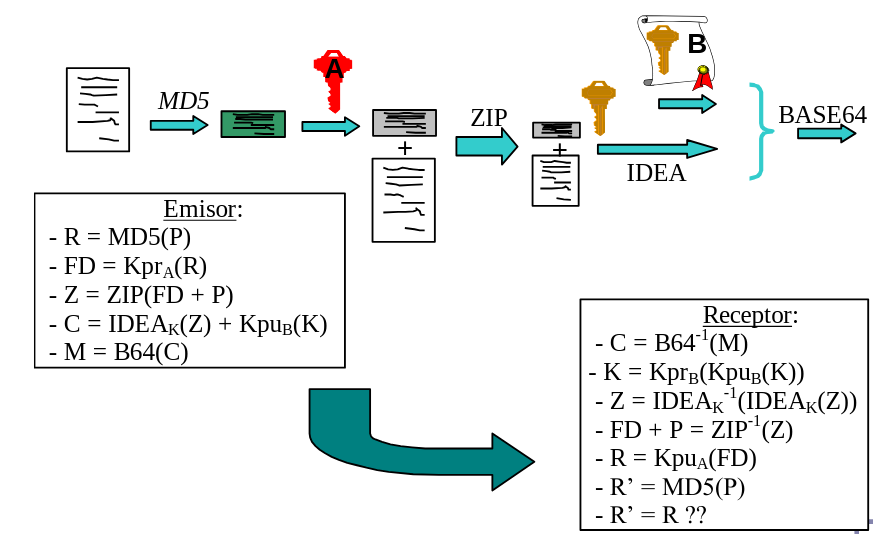
\includegraphics[width=0.8\textwidth]{images/pgp.png}
    \caption{Pretty Good Privacy (PGP).}
\end{figure}

\subsubsection*{Proceso de Cifrado y Descifrado en PGP}

PGP (Pretty Good Privacy) es un método de cifrado para la comunicación segura por correo electrónico. A continuación se detalla el proceso de cifrado y descifrado utilizado en PGP.

\subsubsection*{Cifrado por el Emisor}
\begin{enumerate}
    \item \textbf{Generación de Resumen}: Se genera un resumen del mensaje original \(P\) usando el algoritmo MD5:
    \begin{equation}
        R = \text{MD5}(P)
    \end{equation}
    \item \textbf{Firma Digital}: Se cifra el resumen utilizando la clave privada del emisor \(K_{\text{prA}}\):
    \begin{equation}
        FD = K_{\text{prA}}(R)
    \end{equation}
    \item \textbf{Compresión}: Se comprimen la firma digital y el mensaje original:
    \begin{equation}
        Z = \text{ZIP}(FD + P)
    \end{equation}
    \item \textbf{Cifrado del Mensaje}: Se cifra el mensaje comprimido usando el algoritmo IDEA y una clave de sesión \(K\). Además, se cifra la clave de sesión usando la clave pública del receptor \(K_{\text{pubB}}\):
    \begin{equation}
        C = \text{IDEA}_K(Z) + K_{\text{pubB}}(K)
    \end{equation}
    \item \textbf{Codificación Base64}: El mensaje cifrado se codifica en formato Base64 para su transmisión:
    \begin{equation}
        M = \text{B64}(C)
    \end{equation}
\end{enumerate}

\subsubsection*{Descifrado por el Receptor}
\begin{enumerate}
    \item \textbf{Decodificación Base64}: El receptor decodifica el mensaje del formato Base64:
    \begin{equation}
        C = \text{B64}^{-1}(M)
    \end{equation}
    \item \textbf{Descifrado de la Clave de Sesión}: El receptor descifra la clave de sesión usando su clave privada \(K_{\text{prB}}\):
    \begin{equation}
        K = K_{\text{prB}}(K_{\text{pubB}}(K))
    \end{equation}
    \item \textbf{Descifrado del Mensaje}: Se descifra el mensaje comprimido usando la clave de sesión:
    \begin{equation}
        Z = \text{IDEA}_K^{-1}(C)
    \end{equation}
    \item \textbf{Descompresión}: Se descomprime el mensaje para obtener la firma digital y el mensaje original:
    \begin{equation}
        FD + P = \text{ZIP}^{-1}(Z)
    \end{equation}
    \item \textbf{Verificación de la Firma}: Se descifra la firma digital usando la clave pública del emisor \(K_{\text{puA}}\):
    \begin{equation}
        R = K_{\text{puA}}(FD)
    \end{equation}
    \item \textbf{Verificación del Resumen}: Se genera un resumen del mensaje recibido y se compara con el resumen cifrado recibido:
    \begin{equation}
        R' = \text{MD5}(P)
    \end{equation}
    \begin{equation}
        R' \stackrel{?}{=} R
    \end{equation}
\end{enumerate}





\subsection{Transport Layer Security (TLS) / Secure Sockets Layer (SSL)}

El protocolo \textit{Transport Layer Security (TLS)} (anteriormente conocido como \textit{Secure Sockets Layer (SSL)}) proporciona seguridad en las comunicaciones de red a través de la confidencialidad, autenticación e integridad. Se utiliza ampliamente en protocolos como \textbf{HTTPS}, \textbf{IMAPS}, \textbf{SSL-POP} y \textbf{VPN}.

\subsubsection{SSL Record Protocol}

El \textit{SSL Record Protocol}\footnote{Para ver imágenes sobre este apartado revisa las diapositivas 33 y 34 del tema 4} encapsula los datos de otros protocolos y ofrece un canal seguro que garantiza:

\begin{itemize}
    \item \textbf{Privacidad:} A través de la encriptación de los datos.
    \item \textbf{Autenticación:} Garantizando que el servidor es quien dice ser.
    \item \textbf{Integridad:} Usando técnicas de hash para asegurar que los datos no sean modificados durante la transmisión.
\end{itemize}

Este protocolo se encarga de fragmentar, comprimir y cifrar los datos antes de su transmisión a través de la red.

\subsubsection{SSL Handshake Protocol}

El \textit{SSL Handshake Protocol} es el proceso mediante el cual el cliente y el servidor negocian los parámetros de seguridad antes de la transmisión de datos. Este protocolo realiza las siguientes funciones clave:

\begin{itemize}
    \item \textbf{Negociación del algoritmo de cifrado:} El cliente y el servidor acuerdan qué algoritmo de cifrado utilizar para proteger la comunicación.
    \item \textbf{Negociación de la función hash:} Se selecciona la función hash que se utilizará para garantizar la integridad de los datos.
    \item \textbf{Autenticación del servidor:} El servidor se autentica utilizando un certificado X.509, lo que permite al cliente verificar su identidad.
\end{itemize}

\subsubsection{Generación de Claves de Sesión}

Durante el proceso de \textit{handshake}, se generan las claves de sesión necesarias para proteger la comunicación. Estas claves se generan de la siguiente manera:

\begin{itemize}
    \item \textbf{Claves aleatorias cifradas con la clave pública del servidor (KPUB\_SERVER):} El cliente genera claves de sesión aleatorias que son cifradas con la clave pública del servidor para asegurar su confidencialidad.
    \item \textbf{Diffie-Hellman:} Alternativamente, se puede utilizar el protocolo Diffie-Hellman para intercambiar de manera segura una clave compartida sin necesidad de transmitirla directamente.
\end{itemize}

\subsubsection{SSL Assert Protocol}

El \textit{SSL Assert Protocol} es utilizado para informar sobre cualquier error o anomalía detectada durante la sesión, asegurando que las partes involucradas puedan reaccionar ante posibles problemas de seguridad.

\subsubsection{Change Cipher Spec Protocol}

El \textit{Change Cipher Spec Protocol} notifica cualquier cambio en la configuración del cifrado durante una sesión SSL/TLS. Este protocolo se utiliza para asegurarse de que tanto el cliente como el servidor estén de acuerdo en los cambios realizados en los parámetros de cifrado, como el algoritmo o las claves de sesión.

\subsubsection{Protocolos Utilizados con TLS/SSL}

TLS/SSL es utilizado en una variedad de protocolos para asegurar la comunicación. Algunos ejemplos incluyen:

\begin{itemize}
    \item \textbf{HTTPS:} Protocolo de transferencia de hipertexto seguro utilizado para comunicaciones seguras en la web.
    \item \textbf{IMAPS:} Protocolo de acceso a mensajes de internet seguro, utilizado para acceder a correos electrónicos de manera segura.
    \item \textbf{SSL-POP:} Protocolo de oficina de correos seguro, usado para acceder a correos electrónicos en servidores POP.
    \item \textbf{VPN:} Redes privadas virtuales que utilizan TLS/SSL para crear túneles seguros entre redes.
\end{itemize}




\subsection{IPSec}

El objetivo principal de \textit{IPSec}\footnote{Para ver imágenes sobre este apartado revisa las diapositivas 36 del tema 4} es garantizar la \textit{autenticación}, \textit{integridad} y, opcionalmente, la \textit{privacidad} a nivel de la capa IP. Este conjunto de protocolos se utiliza para asegurar las comunicaciones a través de redes IP, proporcionando confidencialidad e integridad en los datos.

\subsubsection{Procedimientos de IPSec}

IPSec se compone de tres procedimientos clave:

\begin{enumerate}
    \item \textbf{Establecimiento de una Asociación de Seguridad:} 
    \begin{itemize}
        \item Utiliza el protocolo \textit{IKE (Internet Key Exchange)} especificado en la \textbf{RFC 2409}.
        \item El objetivo es establecer una clave secreta compartida entre los participantes, usando el protocolo \textit{Diffie-Hellman}.
        \item Incluye una autenticación previa de los participantes, mediante certificados, para evitar el ataque de \textit{hombre en el medio}.
        \item La asociación de seguridad es \textit{simplex}, lo que significa que tiene un único sentido, es decir, se establece para un único flujo de datos.
        \item La asociación se identifica mediante la combinación de la IP de origen y un \textit{Security Parameter Index (SPI)} de 32 bits.
        \item Una de las limitaciones de este procedimiento es que vulnera el carácter \textit{no orientado a conexión} de la capa IP.
    \end{itemize}

    \item \textbf{Garantizar la Autenticación e Integridad de los Datos:} 
    \begin{itemize}
        \item Se utiliza el protocolo de \textit{Cabeceras de Autenticación} especificado en la \textbf{RFC 2401}.
        \item Este protocolo asegura que los datos transmitidos no hayan sido alterados y autentica a los participantes en la comunicación.
    \end{itemize}

    \item \textbf{(Opcional) Garantizar la Autenticación, Integridad y Privacidad de los Datos:} 
    \begin{itemize}
        \item Se utiliza el protocolo de \textit{Encapsulado de Seguridad de la Carga} especificado en la \textbf{RFC 2411}.
        \item Este protocolo garantiza tanto la integridad como la confidencialidad de los datos, cifrando la carga útil de los paquetes.
    \end{itemize}
\end{enumerate}

\subsubsection{Modos de Operación de IPSec}

IPSec puede operar en dos modos diferentes, según el alcance de la protección que se desea ofrecer:

\begin{itemize}
    \item \textbf{Modo Transporte:} 
    \begin{itemize}
        \item En este modo, la asociación de seguridad se establece entre el host de origen y el host de destino de forma directa, asegurando los datos a nivel de la comunicación entre estos dos puntos finales.
    \end{itemize}
    \item \textbf{Modo Túnel:} 
    \begin{itemize}
        \item En el modo túnel, la asociación de seguridad se establece entre dos routers intermediarios, de manera que todo el tráfico entre estos routers se encuentra protegido, creando un \textit{túnel} seguro para los datos que se transmiten a través de la red.
    \end{itemize}
\end{itemize}





\end{document}


\newpage
% Referencias
\begin{thebibliography}{99}
\bibitem{Referencia1}
Ismael Sallami Moreno, \textbf{Estudiante del Doble Grado en Ingeniería Informática + ADE}, Universidad de Granada, 2025.
% \bibitem{Referencia2}
% Autor(es), \emph{Título del libro}, Editorial, año.

% \bibitem{Referencia3}
% Autor(es), \emph{Título del documento}, Nombre de la Conferencia, páginas, año.
\end{thebibliography}

\end{document}
